\documentclass[12pt,a4paper,bibtotoc,pointlessnumbers]{scrartcl}
\usepackage[ngerman]{babel}
%\usepackage[german]{polyglossia}
%\selectlanguage{german}
% ##########################################
% PDFLaTeX oder nicht:
\newif \ifPDF                                   
\ifx \pdfoutput \undifined \PDFfalse 
\else \ifnum \pdfoutput >0 \PDFtrue
     \else \PDFfalse         
     \fi     
\fi 
% ##########################################
\usepackage{lmodern} %ersetzt Standarsschrift --> für schönere Textdarstellung im PDF
\usepackage[onehalfspacing]{setspace} %setzt das Dokument in 1,5-fachem Zeilenabstand
\setlength\parindent{0pt}% Setzt den Einzug nach einem Absatz fest (hier auf Null)
\usepackage{microtype}

%\usepackage{csquotes}
%\usepackage[style=acm]{biblatex}
%\addbibresource{Literaur.bib}
\usepackage{bibgerm}
%\usepackage{natbib}

\usepackage[
backend=biber,
style=numeric,
%-verb
sorting=none
]{biblatex}

\addbibresource{BA-JannesBrunner.bib}
%\addbibresource{Bildquellen.bib}
%%\bibliography{Masterarbeit.bib}
%\usepackage{cite}


\usepackage[T1]{fontenc} %für europäischen ASCII-Code (mit Umlauten etc)
\usepackage[utf8]{inputenc} %Legt den Zeichencode fest

\usepackage[babel, german=quotes]{csquotes}

\usepackage[dvips]{graphicx} %damit Bilder eingebunden werden Können
\usepackage{fancyhdr} %Nachfolger zu "fancyheadings" --> legt Layout der Seite fest + hält zusätzliche Befehle und Optionen bereit

%\usepackage[headsepline]{scrlayer-scrpage}
%\automark[section]{subsection}

\usepackage{float} %Objekte, die nicht auf zwei Seiten aufgeteilt werden sollen (z.B. Bilder, Tabellen)
\usepackage{floatflt} %wird für die Umgebung floatfigure benötigt --> Bild kann von text umflossen werden
\usepackage[section]{placeins} %section verhindert, dass Bilder aus section hinausgleiten

\usepackage{amsmath} %für Matheumgebung
\usepackage{amssymb} %Setzt Befehle für Symbole in Symbole um 
\usepackage{amsfonts} %Zusätzliche Schriften und Symbole
\usepackage{exscale} %stellt Befehle für Änderung der Schrift bereit
\usepackage{textcomp}
\usepackage{easymat} % weitere Befehle für Matrizen
\usepackage{enumitem} % Ändern von Listenumgebungen
%\usepackage{paralist}

\usepackage{pdfpages}%erlaubt das einbinden von anderen PDF-Dokumenten (auch einzelnen Seiten) in das Latex-Dokument

\usepackage{etex} %erhöht die Anzahl der Pakete, die geladen werden können

\usepackage[font=small,labelfont=bf,hang]{caption} %für Bild- und Tabellenunterschriften
\addto\captionsngerman
{
	\renewcommand{\figurename}{\small{\textbf{Abb.}}}
	\captionsetup{figurewithin = section}
}
\addto\captionsngerman{
	\renewcommand{\tablename}{\small{Tab.}}}
\captionsetup{tablewithin = section}
\captionsetup{font=small, labelfont=bf}

%\usepackage{subfig}
\usepackage{subcaption}
\usepackage{longtable}% erlaubt Tabellen über mehrere Seiten
\usepackage{tabularx} %Tabellen können größer gemacht werden und und die Spalten sind flexibler
\usepackage{booktabs} %definiert Befehle für Tabellen
%\usepackage{booktabs-de}
\usepackage{ltxtable} %vereinigt longtable und tabularx
\usepackage{colortbl}
\usepackage{multirow}
%\usepackage{multicolumn}
\usepackage{rotating}
%\usepackage{tablefootnote}

%\usepackage{tikz}

\usepackage{array} %erweiterte Möglichkeiten für Tabellen und Spalten
%\usepackage{subfigure}
\usepackage{url} %lange Zeichenfolgen können trotz fehlender Leerzeichen getrennt werden
%\usepackage{paralist}
% ##########################################

% ##########################################
% Seitendesign:
\usepackage{units}
\usepackage[headheight=50pt, a4paper, bottom=25mm, footskip=6mm]{geometry} %wird für Layout des Dokuments benötigt
\geometry{verbose}
% ##########################################
%\usepackage{cite} % fasst Zitate zusammen (funktioniert nur ohne hyperref)

\ifPDF
\usepackage{xcolor}   %ermöglicht das Ändern der Farbe von Schrift, Seitenhintergrund, Boxen etc
\usepackage[
  pdftex,
  colorlinks,
  citecolor = {green},
  linkcolor = {black},
  urlcolor  = {gray},                
  bookmarks         = true,
  bookmarksopen     = true, % Bookmarks anzeigen...
  bookmarksnumbered = true, % ...und numerieren
  pdftitle          = {BA},
  pdfauthor         = {Jannes Brunner}
]{hyperref} %ermöglicht Links im PDF-Dokument (z.B. ancklicken eines Kapitel im Inhaltsverzeichnis oder Verlinkung mit externem Link)


\else
\usepackage{wrapfig}
%\usepackage{floatflt} %ermöglicht Gleitobjekte (Bilder, Tabellen) von Text umfließen zu lassen und Bilder links/recht je nach Seitenzahl auszurichten
\fi%-----------------------------------------------------------------------------
% Definition für einen neuen Befehl für deutsche Anführungszeichen
\newcommand{\gqq}[1]{\glqq{}#1\grqq{}}
\newcommand{\gq}[1]{\glq{}#1\grq{}}


\begin{document}
	\begin{titlepage}
		\begin{center}
%				\begin{figure}[h]
%					\begin{minipage}{.4\textwidth}
%						\centering
%						\includegraphics[width=0.5\textwidth]{Bilder/Logo_Wildau}
%					\end{minipage}
%					\begin{minipage}{.2\textwidth}
%						\hspace{\textwidth}
%					\end{minipage}
%					\begin{minipage}{.4\textwidth}
%						\centering
%						\includegraphics[width=0.4\textwidth]{Bilder/bam_logo_135}
%					\end{minipage}
%				\end{figure}			
%				\vspace{0.4cm}
			
%			{\large \bf Bundesanstalt für Materialforschung und -prüfung }\\[4mm]
%			{\large\bf TH Wildau}
			%\vspace{0.5cm} \hrule \vspace{1.3cm}
			
			 
			\begin{doublespace}
			{\huge Entwicklung einer webbasierten Client-Server Anwendung zur Unterstützung von interaktiven Unterrichtsmethoden}\\
			\end{doublespace}
			\vspace{2cm}
			
			{\huge \bf Bachelorarbeit}\\
			\vspace{0.4cm}
			
			{\large zur Erlangung des akademischen Grades\\ Bachelor\\ (B.-Sc.)\\an der HTW Berlin}\\
			
			\vspace{1cm}
			
			{\Large \bf Hochschule für Technik und Wirtschaft Berlin}\\
			{\large \bf Fachbereich Informatik, Kommunikation und Wirtschaft\\
			Studiengang internationale Medieninformatik}\\
		
			\vspace{1.5cm}
			
			{\doublespacing Eingereicht von\\
			{\Large \bf Jannes Julian Brunner}\\ geb. 21.06.1991}
			
%			\vspace{1cm}
		
			\large
			\begin{table}[b]
				\begin{center}
					\begin{tabular}{ll}
					Eingereicht am:& 29.07.2019\\
					Betreuender Hochschuldozent:& Prof. Dr. Gefei Zhang\\
					Zweitgutachter: & Prof. Dr.-Ing. Kai Uwe Barthel\\
					\end{tabular}
				\end{center}
			\end{table} 
		\end{center}
		\vspace{0.6cm}
	%	{\bf Abstract}: Das Abstract
\end{titlepage}

\newpage
%\clearpairofpagestyles




%\clearpairofpagestyles

\pagenumbering{roman}
\setcounter{page}{10}

\section*{Abstract}\label{sec:abstract}
\newpage

%\thispagestyle{empty}
\cfoot{\pagemark}
\tableofcontents 
\newpage

\pagenumbering{arabic}




%\pagestyle{scrheadings}
%\ihead{\leftmark}
%%\automark{section}
%\chead{\rightmark}
%%\automark{subsection}
%\ohead{\thepage}


\pagestyle{fancy}
\fancyhf{}
%\setlength{\headheight}{15pt}
\renewcommand{\headrulewidth}{0.4pt} %definiert die Dicke der Linie unter der Kopfzeile
%\renewcommand{\footrulewidth}{0pt} %definiert die Dicke der Linie über der Fußzeile
\renewcommand{\sectionmark}[1]{%
	\markboth{\thesection.\ #1}{}} %sorgt dafüpr, dass die Kapitel und Unterkapitel in der Kopfzeile stehen


%\addtolength{\headwidth}{\marginparwidth}
%\setlength{\fancyhead}{0.4\headrulewidth}
\fancyhead[L]{\textsl{\small 
%		\leftmark \hspace{0.8cm}
		\rightmark}}
%\fancyhead[C]{\parbox{0.5\textwidth}{\textsl{\small \rightmark}}}
\fancyhead[R]{\textsl{\small \thepage}}
%\fancyhead[L]{\parbox{0.3\textwidth}{\textsl{\small \leftmark}}}
%\fancyhead[C]{\parbox{0.6\textwidth}{\textsl{\small \rightmark}}}
%\fancyhead[R]{\parbox{0.05\textwidth}{\textsl{\small \thepage}}}
%\addtolength{\headwidth}{\marginparsep}
%\fancyfoot[C]{\thepage}


\thispagestyle{empty}
\section*{Selbstständigkeitserklärung}\label{sec:selbststandigkeitserklarung}
Ich erkläre hiermit, dass ich die vorliegende Bachelorarbeit selbstständig verfasst und dazu  keine  anderen  als  die  angeführten  Behelfe  verwendet,  die  Autorenschaft  eines Textes  nicht  angemaßt  und  wissenschaftliche  Texte  oder  Daten  nicht  unbefugt verwertet habe. Die elektronische Kopie ist mit den gedruckten Exemplaren identisch.
\vspace{5cm}
\\

Berlin, \today, 
\begin{flushleft}
	\line(1,0){350}\\
	(Ort, Datum, Unterschrift)
\end{flushleft}
\newpage

\input{sections/00Begriffe}
\newpage

\section{Einführung}\label{sec:einfuhrung}
\subsection{Motivation}\label{sec:motivation}

Bildung ist ein wichtiges Element der Persönlichkeitsentwicklung und unter Artikel 26 der allgemeinen Erklärung der Menschenrechte als solches definiert. Ohne Bildung ist das Ausüben eines gewählten Berufes und das Entwickeln einer Meinung zu komplexen Sachverhalten unmöglich. \cite{weitblicker.org2019:online}. Heute sieht sich Bildung durch den digitalen Wandel der letzten Jahre sich noch nie vorher dagewesenen Problemen gegenübergestellt. Wie können Lehrende an Schulen digitale Technik effizient und preiswert im Unterricht einsetzen und so neue Bildungskonzepte erfolgreich in den Lehrplan integrieren? Ursprünglich bezeichnet der Begriff Digitalisierung das Umwandeln von Analog nach Digital. Wurde früher Musik auf Schallplatten vertrieben, so wurde diese von der Compact Disc vom Markt verdrängt, welche die Musik auf kleinerem Raum digital abspeichert. Auch wenn der Begriff im Zusammenhang mit Schule längst nicht mehr das Ursprüngliche meint, halte ich es für sehr wichtig, früher dagewesene Unterrichtskonzepte nicht einfach zu digitalisieren sondern es erfordert ein Neudenken. Bewährte pädagogische Methoden sollten durch Digitalisierung profitieren sowie neue Konzepte müssen erforscht und entwickelt werden. 

\subsubsection{Besuch Grundschule am Rüdesheimer Platz Berlin}\label{sec:grundschulebesuch}
Im Rahmen der Vorrecherche zu dieser Arbeit wurde einem Unterrichtstag in 
einer Jahrgangsübergreifenden (JüL) Klasse 1 bis 3 an der Grundschule am Rüdesheimer Platz beigewohnt um ein differenzierteres 
Bild der gegenwärtigen Lern- und Digitalisierungssituation an einer Berliner Schule zu bekommen. An dieser Stelle eine große Dankaussagung an Frau Wewer, Grundschullehrerin, welche diese Erfahrung möglich gemacht hat und in einem anschließenden Gespräch das Interesse an einer kostengünstigen und einfach nutzbaren Lösung zur Unterstützung von interaktiven Unterrichtsmethoden unterstrichen hat.
\newpage
\subsection{Problemstellung}\label{sec:problemstellung}
%Kurze Zusammenfassung des Forschungsstandes genügend?
Am 04.04.2019 trat die Änderung des Art. 104c des Grundgesetz für die Bundesrepublik Deutschland in Kraft
und ebnete so den Weg für den von Bund und Ländern beschlossenen Digitalpakt Schule \cite{Art104cG55:online}. 
Dieser Beschluss macht deutlich, dass digitale Kompetenz im Bildungssektor von hoher Bedeutung ist, was auch von einer Förderungssumme von mindestens 5,5 Milliarden Euro unterstrichen wird. 
Legt man diese Summe auf die ca 40.000 Schulen um, erhält jede Schule einen Durchschnittsbeitrag von 137.000 Euro. Bei ca. 11 Millionen Schülerinnen und Schülern würde das eine Förderungssumme von ca. 500 Euro pro Schülerin bzw. Schüler bedeuten. 
Einer der Hauptförderungspunkte des Digitalpakt Schule sieht den Ausbau der technischen Infrastruktur
an deutschen Schulen vor, z.B. Bereitstellung von drahtlosen Netzwerken, schnellen Internetzugangspunkten und digitale Unterrichtsmedien wie interaktive Whiteboards.
\\ \\
Das Bundesministerium für Bildung und Forschung (BMBF) gegenargumentiert damit, dass kein digitales Medium alleine gute Bildung fördert, sondern immer dahinterstehende pädagogische Konzepte aus einer Vielfalt von Angeboten entscheidend sind. \cite{dpakt2019:online} Ergänzend dazu kritisiert Dennis Horn (Experte für digitale Themen der ARD) den zu starken Fokus auf Hardware und mahnt an, dass zu wenig darüber gesprochen wurde, wie diese denn auch sinnvoll genutzt werden kann.\cite{Horn2018:online}. \\ \\
Diese Kritikpunkte wurden auch auf der Podiumsdiskussion der re:publica 2018 - 'Was kommt in den digitalen Schulranzen?' angeschnitten. Tobias Hübner, Lehrer und Autor im Bereich Medienistik, zeigt dort ebenfalls auf, dass der Wille Geld auszugeben zu begrüßen sei, es aber an Konzepten und Materialien mangele. Als Lehrer würde er den Investitionsfokus auf Lehrerfortbildung setzen.
\\ \\

Der populäre Tablet Computer 'iPad' der Firma Apple inc. kostet in der günstigsten Variante bereits mindestens 449€ \cite{iPadmini65:online} (Stand April 2019), was schon knapp 90\% des Förderungsvolumens pro Schülerin und Schüler ausmachen würde. Als ein Gegensatz wäre hier der Einplatinencomputer Raspberry Pi zu nennen, welcher bereits für 33 Euro erwerblich ist (Stand April 2019) und genug Rechenkapazitäten bereitstelle um zahlreiche Projekte im Bildungsbereich durchzuführen. Mit Touchscreenmodul und Schutzhülle liegt der Preis insgesamt bei ca. 150 Euro, was immer noch weniger als die Hälfte des Fördervolumens beträgt. 

\begin{figure}[H]
	\centering
	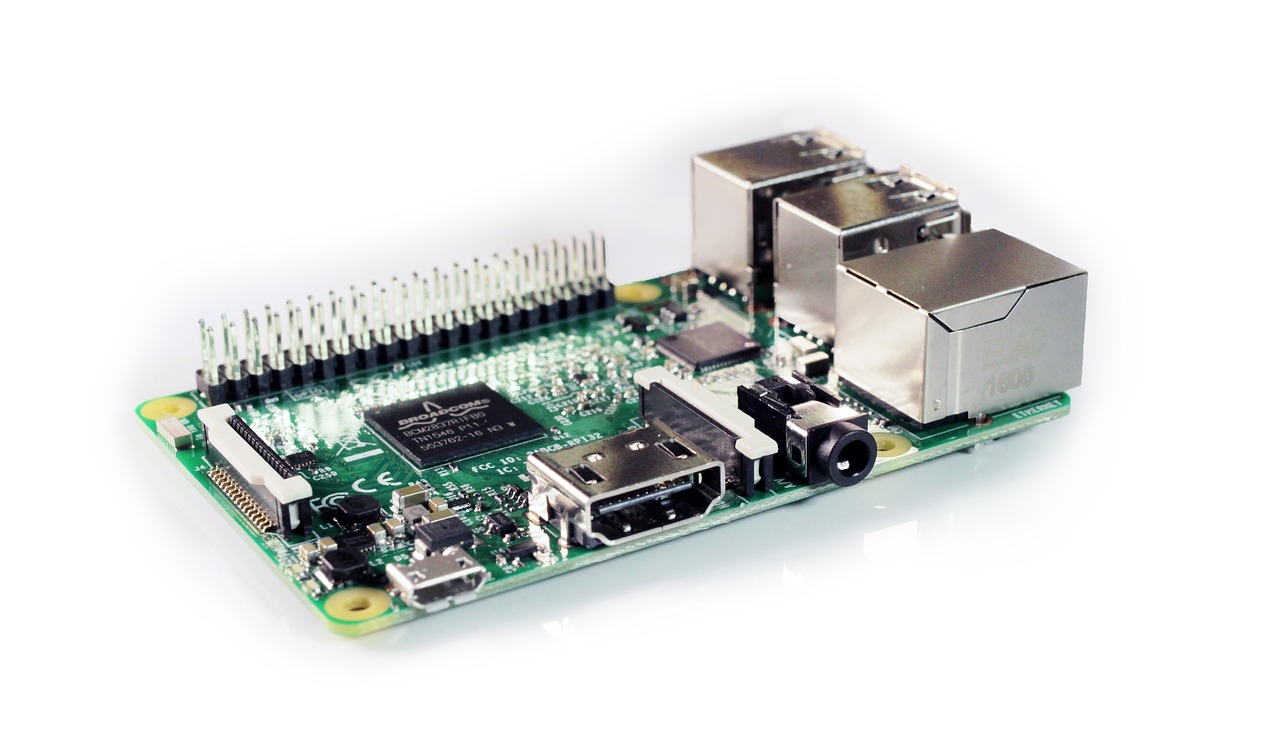
\includegraphics[width=0.8\linewidth]{bilder/raspberry-pi}
	\caption[Raspberry Pi 3 - Einplantinencomputer]{Der Raspberry Pi 3 - Einplantinencomputer \cite{PixaPi2016}}
	\label{fig:server_diagram}
\end{figure}


\subsection{Zielsetzung}\label{sec:zielsetzung}
Seit dem Erfolgskurs des Web 2.0\footnote{Web 2.0 ist ein Schlagwort, das für eine Reihe interaktiver und kollaborativer Elemente des Internets, speziell des World Wide Webs, verwendet wird. Dabei konsumiert der Nutzer nicht nur den Inhalt, er stellt als Prosument selbst Inhalte zur Verfügung. - Wikipedia.org} in den frühen 2000er Jahren, zeichnet sich zunehmend der Trend des Software-as-a-Service Geschäftsmodells ab. Dies beschreibt die Bereitstellung von Software im Internet oder durch ein lokal laufenden Servers, ohne dass Benutzende die Software selbst noch lokal installiert haben müssen. Im Jahr 2015 setzten bereits über drei Viertel von 102 befragten Unternehmen Software dieser Form aktiv im Geschäft ein\cite{TecArt-GmbH2019:online}. Viele Arten von Software können  mittlerweile in einer im Webbrowser lauffähigen Alternative substituiert werden. Ein populäres Beispiel ist die Office-Suite Google Docs der Firma Google inc. Hier lassen sich Textverarbeitung, Tabellenkalkulation und das erstellen von Präsentationen ohne Installation und direkt im Webbrowser des Benutzenden ausführen. Ein anderes Beispiel ist die Web-Software Photopea welche ebenfalls komplett im Web-Browser ausgeführt wird und dem nur lokal installiert ausführbaren quasi Industriestandard Bildbearbeitungsprogramm Photoshop der Firma Adobe inc. sehr nahe kommt. Im Vergleich zu lokal installierter Software ist die Bereitstellung von Web-Software einfacher, da solange ein moderner Webbrowser lauffähig ist, das Betriebssystem des Client-Computers zu vernachlässigen ist. Ebenso stellt potente Hardware keine zwingende Voraussetzungen, da etwaige rechenintensive Aufgaben auf der Serverseite getätigt werden können oder hier eine Balance zwischen Client und Server angestrebt werden kann. \\ 
% Das da oben noch Teil der Problemstellung?
%Hier jetzt Web Trend noch erwähnen!
Ein Raspberry Pi Einplantinencomputer bietet bereits genügend Leistung für Webtechnologien und ein günstigen Anschaffungspreis. Auch besitzen bereits 67\% der 10-11 jährigen Jugendlichen ein Smartphone \cite{Statista2017:online} welches ebenfalls genug Leistung für Webanwendungen aufweisen. \\ \\ Eine Softwarelösung zur Unterstützung von interaktiven Unterrichtsmethoden, welche auf Webtechnologien basiert, könnte den Rahmen der im Digitalpakt Schule fließenden Gelder optimierter ausschöpfen und Schulen finanzielle Flexibilität einräumen. 
\\ \\
Diese Arbeit wird sich der Thematik von pädagogischen digitalen Konzepten und Varianten von interaktiven Unterrichtsmethoden nur im Rahmen der Softwareentwicklung widmen und ihre forschungsrelevante Tiefe nicht gänzlich erfassen, da dies den Rahmen der Zielsetzung überschreiten würde.

%wichtigste Quellen hier noch nennen un
\newpage

\subsection{Aufbau der Arbeit}
Im Anschluss an dieses Kapitel werden \hyperref[sec:grundlagen]{\textbf{Grundlagen}} erörtert. Dies umfasst die Themengebiete Digitalisierung an Schulen und einen Überblick über Webtechnologie. Ersteres ist für den späteren potentiellen Einsatz der Software maßgebend, letzteres bildet das technologische Fundament, welches die Implementierung erst möglich macht. Anschließend wird in Kapitel \hyperref[sec:analyse]{\textbf{Analyse}} ein Vergleich zwischen existierenden kommerziellen und nicht-kommerziellen Plattformen gezogen. Darauf aufbauend folgt eine Anforderungs- und Systembeschreibung. Im darauffolgenden Kapitel \hyperref[sec:konzept]{ \textbf{Konzept}} wird ebendieses erörtert und darauffolgend der Prozess der \hyperref[sec:implementierung]{\textbf{Implementierung}} beschrieben. In einer folgenden \hyperref[sec:auswertung]{\textbf{Auswertung}} werden die Ergebnisse mit den geplanten Zielen verglichen und ein Fazit gezogen. Schlussendlich wird im letzten Abschnitt ein \hyperref[sec:ausblick]{\textbf{Ausblick}} formuliert, welcher die Zukunft des Projekts betrifft. 
   

\newpage

\section{Grundlagen}\label{sec:grundlagen}
Dieses Kapitel soll einen grundlegenden Überblick über die zwei wichtigsten Themen dieser Arbeit bieten, Dclearigitalisierung an Schulen und der damit verbundene Einsatz von digitalen Unterrichtsmethodiken
\subsection{Digitalisierung an Schulen}
\subsubsection{Digitale Technik im Unterricht}\label{sec:technikunterricht}
\subsubsection{Ausblick Interaktive Unterrichtsmethoden}\label{sec:interaktiveunterr}
\subsubsection{Datenschutz an Schulen}\label{sec:datenschutz}

\subsection{Überblick Webtechnologie}\label{sec:webbasedsoftware}
% Hier auf PDF Technische Anforderungen verweisen (Footnote?) da sehr ausführlich und gut
% Anfang Geschichtlich
Diese Sektion soll einen grundlegenden über im Kontext dieser Arbeit wichtigen Begrifflichkeiten bieten. Die folgenden Untersektion 2.2.1 ff. werden die Thematiken nur grob umreißen, da eine detaillierte Betrachtung der genannten Begriffe den Rahmen dieser Arbeit weit überschreiten würde. 

\subsubsection{Intranet und Internet}\label{sec:intranetundinternet}
% Detailgrad so sinnvoll?
% Unterschied und Gemeinsamkeit klar machen
% Hier kommunikation erklären! Protokolle und OSI schicht!
Einfach ausgedrückt, ist das Internet ein Netzwerk von Computern, welche weltweit miteinander vernetzt sind. Seine Anfänge lassen sich auf das Ende der 1960er in den USA datieren, als die DARPA (Defense Advanced Research Projects Agency) eine weltweite Verknüpfung von Datennetzen anstrebte. Das hier draus resultierende ARPANET (Advanced Research Projects) kann als Ursprung angesehen werden. Dabei beschreibt der Begriff Internet streng genommen ein 'interconnected network', also ein international vernetztes Netzwerk, ohne dabei die Hardware- und Netzwerktechnologie genauer zu beschreiben \cite{safran2011webtechnologien:article}.  \\ 
Der wohl populärste Anwendung des Internets ist das World Wide Web, welche gegen das Jahr 1989 von einer Forschungsgruppe rund um Sir Tim Berners-Lee ins Leben gerufen wurde und heute oftmals als Synonym für das gesamte Internet sprachlich genutzt wird. \\ 

In unser heutigen globalisierten Welt lässt sich das Internet mitsamt World Wide Web nicht mehr wegdenken und ist ein integraler Bestandteil der Informationskultur. 
 \\ \\
 Das Intranet beschreibt analog dazu ein lokal abgeschlossenes Netzwerk von Computern, bspw. innerhalb eines Unternehmens. Dabei endet ein Intranet klar an seinen Grenzen und ein Gateway fungiert als Übergabepunkt ins Internet. Die Vernetzung der Endgeräte erfolgt kabelgebunden (LAN) oder kabellos (WLAN). Die Kommunikationsgeschwindigkeit innerhalb eines Intranets sind i.d.R. deutlich höher als im Internet, da Daten nicht erst nach außen an einen Internet Service Provider übermittelt werden müssen. Ein Intranet funktioniert unabhängig vom öffentlichem Internet (erhöhte Ausfallsicherheit), ist nicht öffentlich zugänglich und bietet oft andere oder zusätzliche Funktionen. \cite{Intranet62:online}. 
 
 \subsubsection{Client-Server Modell}\label{sec:clientservermodell}
 Das Client-Server Modell beschreibt das Prinzip der Kommunikation zwischen zwei Teilnehmer innerhalb eines Netzwerks. Grundlegend unterscheidet das Modell hierbei zwischen einer Anbieterseite (Server) und einer Benutzerseite (Client). Der Client betreibt auf seinem Endgerät (Computer, Smartphone, etc.) eine Clientsoftware mit der die Verbindung zum Server aufgebaut wird. Im Fall des WWW (siehe \ref{sec:www}) ist dies in den meisten Anwendungsszenarien ein Webbrowser. Der Client fordert dabei eine Resource an, welche auf dem Server vorliegt oder dort speziell für die Anfrage des Clients generiert wird (siehe auch Sektion \ref{sec:webanwenservices}). Das Client-Server Modell sieht vor, dass immer der Client die Verbindung aufbaut, nie andersherum \cite{ElektronikKompendium.de:online}. Die Anfrage des Clients wird Request genannt, die Antwort des Servers Response oder Reply, welche bei ausreichender Berechtigung des Clients auch Daten enthält. 
 Server-Computer sollen rund um die Uhr erreichbar sein, während Client-Endgeräte auch abgeschaltet werden können, ohne die Integrität des Netzwerks zu beeinflussen. 
  % Vergleich zu anderen Modellen?
 
\subsubsection{Kommunikation}\label{sec:kommunikation}
Die Kommunikation im Internet und Intranet erfolgt über Protokolle. 
Ein Protokoll kann als ein Satz von Kommunikationsregelvorschriften verstanden werden \cite{safran2011webtechnologien:article}, welche den Netzwerkverkehr auf unterschiedlichen Schichten reglementieren. 
Diese Schichten werden im OSI-Modell (Open System Interconnection) der ISO (International Standardization Organisation), der internationalen Standardisierungsorganisation beschrieben. (Siehe Tabelle) %HIER TABELLE!
\\ 
Das OSI-Modell ist dabei in sieben Schichten eingeteilt, während die Erste als physikalische Schicht definiert ist und die Siebte als Anwendungsschicht. Protokolle sind dabei jeweils nur über Protokolle benachbarter Schichten in Kenntnis gesetzt. Das OSI-Modell lässt sich grob in anwendungsorientierte Schichten (1 bis 4) und transportorientierte Schichten (5 bis 7) unterteilen. Die im Rahmen dieser Arbeit genutzten Webtechnologien nutzen kommunikativ nur anwendungsorientierte Schichten des ISO-OSI Modells.



% Begriff Internet
\subsubsection{World Wide Web}\label{sec:www}
Das World Wide Web (WWW) ist die wohl populärste Anwendung des Internets \cite{safran2011webtechnologien:article} und wird oftmals fälschlicherweise als Synonym für das gesamte Internet genannt. Das WWW ist eine Sammlung von verteilten Dokumenten, welche sich gegenseitig über sog. Hyperlinks referenzieren und von Web-Servern zur Verfügung gestellt werden. Auf der Client Seite (siehe \ref{sec:clientservermodell}) stellt der Web-Browser die wichtigste Software da. Mit ihr werden Web Server angesprochen (Request) und Antworten (Response) für den Nutzenden dargestellt. Die wichtigsten sprachlichen Komponenten des WWW sind: \\ 
\begin{itemize}
	\item HTML: Hypertext Markup Language - eine reine Beschreibungssprache, welche Hypertext Dokumente durch Tags codiert. 
	\item CSS: Cascading Style Sheet - Eine Stylesheet Sprache, welche das äußere Erscheinungsbild von Hypertext Dokumenten beschreibt
	\item JS: JavaScript: Eine Skriptsprache, welche u.A. Interaktion sowie Dynamik hinzufügt und clientseitig interpretiert wird. 
\end{itemize}
Die Techniken des WWW können auch lokal im Intranet genutzt werden. 
Das zur Verständigung zwischen Client und Server genutzte Protokoll (siehe \ref{sec:kommunikation})ist das Hypertext Transfer Protocol (HTTP) bzw. in verschlüsselter Form Hypertext Transfer Protocol Secure, da eine Übermittlung im Klartext nicht immer wünschenswert ist. HTTP/HTTPS ist ein Zustandsloses Protokoll, das bedeutet dass jede Anfrage unabhängig voneinander geschieht und betrachtet wird. Dies und die Tatsache, dass jede Anfrage von der Client-Seite aus gestartet werden muss (siehe \ref{sec:clientservermodell}), stellen oftmals Hürden für die Entwicklung von Webanwendungen und Webservices da. Techniken wie Cookies und Sessions, sowie das wiederholte Abfragen von aktualisierten Daten seitens des Clients wirken hier entgegen. Cookies stellen persistent gespeicherte Daten auf der Client-Seite da, mit deren Hilfe der Webserver einen Client eindeutig zuordnen kann. Bei einer Session sendet der Client bei jeder Anfrage eine eindeutige ID an den Server. Im Normalfall endet eine Session beim Beenden des Webbrowser, während Cookie-Dateien eine längere Lebensdauer besitzen.      
%
\subsubsection{Webanwendungen und Webservices}\label{sec:webanwenservices}
Im Laufe der Entwicklung des WWW (\ref{sec:www}) stieg der Anspruch vom reinen Anbieten statischer Dokumenten in Richtung dynamischer Inhalte, welche einer Programmlogik folgend von einem Webserver für jede Anfrage generiert werden. Webanwendungen sind Computerprogramme, welche auf einem Webserver ausgeführt werden und den Webbrowser des Clients als Schnittstelle nutzen \cite{safran2011webtechnologien:article}. Dies bietet den großen Vorteil, dass etwaige Anpassungen von Programmlogik nur serverseitig erfolgen müssen und jeder Client mit Webbrowser als Benutzerschnittstelle ausreicht. \\ \\
Webservices sind eine spezialisierte Art von Webanwendung. Die Fokus hier liegt auf das bereitstellen von Daten für andere Applikationen, welche die gewonnen Daten selbst auswerten und dem Nutzenden bereitstellen. Dies geschieht i.d.R. über eine einheitlich beschriebene Schnittstelle (API - Application Programming Interface), über welche fremde Applikationen angefragte Daten abrufen können. Der Austausch der Daten erfolgt hier meist über Formate wie JSON (JavaScript Object Notation) oder XML (Extensible Markup Language), da Aussehen und Lesbarkeit der Daten irrelevant sind und somit eine Ausgabe in HTML nicht von Nöten ist. \\
Bei der Implementierung eines Webservices bieten sich folgende zwei technologische Arten der Umsetzung an: \\ \\
\textbf{SOAP/WSDL}: Hier werden Nachrichten über das Simple Object Access Protocoll ausgetauscht (SOAP) und deren Beschreibung über die Web Services Description Language (WSDL) definiert. Anfrage- und Antwortformat der Daten ist XML (Extensible Markup Language), eine Auszeichnungssprache, welche HTML sehr ähnelt aber deutlich allgemeiner ist. XML kann als mehr als Regelwerk verstanden werden, mitdessen Hilfe Entwickler ihre eigene hierarische Beschreibung einer Datenstruktur vornehmen können. XML und HTML leiten sich bei der von der SGML (Standard Generalized Markup Language) ab, welches ihre Ähnlichkeit zusätzlich herleitet \cite{XMLHTMLU88:online}. \\

 
\textbf{REST}: (Representational State Tranfer) Hier kann jede einzelne Funktion des Webservices über eine jeweils zugeordnete URL abgerufen (Uniform Resource Locator) werden, umgangssprachlich als Webadresse bekannt. Das WWW selbst kann als REST-Webservice verstanden werden \cite{Bayer2002:online}. \\ 

\subsection{Websockets}\label{sec:websockets}
Bezugnehmend auf die Problematik, welche durch die Kommunikationsstrategie über das http-Protokoll entsteht (siehe Sektion \ref{sec:www}), wirken Websockets dieser entgegen. Als Kommunikationskanal verknüpft ein Websocket Server und Client. Zwar muss die Kommunikation zunächst über den Client initiiert werden, bleibt dann jedoch bestehen und der Server kann diese nutzen um aktiv neue Daten zu emittieren. Ein Nachteil ist jedoch, dass im Gegensatz zum http-Protokoll hier auch Daten hin- und hergeschickt werden, wenn dies eventuell nicht gewünscht ist \cite{neumann2015entwicklung}, was insbesondere bei mobilen Applikationen kritisch sein kann. 

\subsection{Webapplikationsentwicklung}\label{sec:softwareentwicklung}
Dieses Kapitel soll den wesentlicheren Bestandteil dieser Arbeit grundlegend beleuchten, der Entwicklung von Webapplikationen.
Webanwendungen und Webservices können unter diesem Begriff zusammengefasst werden.
 \\ 
\subsubsection{Web-Application-Frameworks} \label{sec:wafs}
Bei der Entwicklung von Webapplikationen wird oftmals auf Frameworks (z.Dt. Rahmengerüste), spezifischer Web-Application-Framework (WAF) zurückgegriffen. 
Ein WAF bezeichnet damit ein Programmgrundgerüst, welches als Grundlage zum Einsatz kommt \cite{Ionis2019:online}. Dies erleichtert die Entwicklung ungemein, da auf bereits vorgefertigte Ansätze und Programmbausteine zugegriffen werden kann und diese nicht selbst von Hand implementiert werden müssen. Diese WAFs reflektieren zumeist auch eine Modelle und Prinzipien, welche, falls dem Entwickelnden bekannt, den Einstieg erleichtern. 
Ein für Frameworks bekanntes Paradigma stellt das Umsetzungsparadigma \\
\textbf{Inversion of Control} (IoC), z.Dt. Umkehrung der Steuerung da, welches u.a. auch in der objektorientieren Programmierung Anwendung findet.
Hierbei wird eine Funktion/Unterprogramm bei der Hauptprogrammbibliothek registriert und von dieser zu einem späteren Zeitpunkt aufgerufen. Dies ist umgangssprachlich auch als 'Hollywood'-Prinzip bekannt ('Don't call us! We call you' z.Dt. 'Ruf nicht uns an! Wir rufen dich an!'). Das Framework behält also die Programmflusssteuerung bei. 
  Ein Nachteil, der durch dein Einsatz von einem WAF bedingt ist, stellt die Einschränkung der Freiheit während des Implementierungsprozesses da, dieser wird jedoch billigend in Kauf genommen, da sich ein Reduktion des Zeit- und Kostenaufwands erhofft wird. Die Wahl des richtigen WAF ist ein wichtiger Entschcheidungsprozess, bei dem mehrere Faktoren beachtet werden müssen, wie z.B. benötigte Einarbeitungszeit und Lizenzen.

\subsubsection{Serverseitiger Ansatz}\label{sec:serverseitgeransatz}
Anknüpfend an Sektion \ref{sec:webanwenservices}, sind Webapplikationen Software, welche Serverseitig ausgeführt werden, wobei der Webbrowser eines Nutzenden als Benutzerschnittstelle dient. Eine Webapplikation kann jedoch auch clientseitig implementiert werden, wie in Sektion \ref{sec:clientseitigeransatz} beschrieben. \\ \\
Serverseitige Webapplikationen verfolgen oftmals den Multi-Page Ansatz, das heiß pro Anfrage (Request) wird eine anderes Dokument dem Client (Webbrowser) übergeben. Wichtige Programmiersprachen für den Ansatz sind php, Ruby, Python, Java und auch JavaScript, was vorher zunächst nur auf der Clientseite zur Anwendung kam. \\
Die \textbf{Model - View - Controller} Architektur (MVC) ist vorherrschende Architektur, auf welche sich der Großteil der serverseitigen WAFs stützen.
Hierbei wird die Programmlogik klar in drei große Bestandteile unterteilt: \\
\textbf{Model}: Das Model oder z. Dt. Modell beschreibt eine Datenstruktur an sich. In einem Webshop wären dies z.B. die Produkte und deren Eigenschaften wie ID, Name, Preis usw. \\
\textbf{View}: Diese beschreibt die reine Ansicht eines Dokuments. In einem Webshop wäre dies z.B. die Detailseite eines Produkts. Dabei sollte so wenig wie nötig Logik selbst im Code der View vorkommen. \\
\textbf{Controller}: Der Controller dient als Bindeglied zwischen Model und View. Er handelt ankommende Requests (Anfragen) ab und übergibt der View aus dem Modell die notwendigen Daten. \\ 
Neben der MVC Architektur existieren weitere, andere Architekturen und Ableitungen der MVC Architektur, wie z.B. der im Django WAF genutzten Model - View - Presenter Architektur. \\
Es folgt eine Tabelle, die einen groben Überblick über bekannte WAFs, welche den serverseitigen Multi-Page Ansatz verfolgen \cite{TopWebDe0:online}. 

\begin{table}[H]
	\centering
	\caption{Überblick serverseitiger Web-Application-Frameworks}
	\label{tab:spektrometer}
	\begin{tabular}{lcc}
		\textbf{Name} & \textbf{Sprache} & \textbf{Architektur}   \\ 
		\hline 
		Symfony & php & Model - View - Controller \\
		Laravel	& php & Model - View - Controller  \\ 
		Phalcon	& php & Model - View - Controller   \\ 
		Codeigniter & php & Model - View - Controller \\
		Django & Python & Model - View - Presenter \\		
		Ruby on Rails & Ruby & Model - View - Controller \\
		\hline 
	\end{tabular} 
\end{table}


Aus der Tabelle lässt sich eine starke Popularität der Programmiersprache php ableiten und deren auf dieser Sprache basierenden WAFs. Die Tabelle stellt keinen Anspruch auf Vollständigkeit, da noch unzählig viele andere serverseitige WAFs existieren, die den Rahmen der Tabelle überschreiten würden. Ebenso wurde das WAF ExpressJS, welches auf der serverseitigen Plattform NodeJS basiert, bewusst nicht mit in die Tabelle aufgenommen, da dies ein Sonderfall darstellt. Diese Thematik wird in Kapitel \ref{sec:konzept} ausführlich behandelt. 
%Hier über NodeJS und PHP quatschen!
\subsubsection{Clientseitiger Ansatz}\label{sec:clientseitigeransatz}
 Das Programmiermodell des WWW, welches durch die Architektur des Hypertext Transfer Protocol (HTTP) geprägt ist, wird bei der Entwicklung von Webapplikationen übernommen. Dies sieht eine Anfrage immer seitens des Clients vor (siehe auch Sektion \ref{sec:www}). Dies schränkt das Ausmaß von Interaktion und generieren von dynamisch ladenden Webseiten ein. 
 Der clientseitige Ansatz der Webapplikationsentwicklung kommt meistens bei sog. Single-Page Applikationen zutrage. Hierbei wird o.g. Problem damit umgangen, indem bei Aufruf einer Internetseite die gesamte HTML Benutzeroberfläche inklusive Programmlogik in Form von JavaScript Code als Ganzes an die Client übergeben wird. Dies bietet den großen Vorteil, dass die Logik nun auf dem Client ausgeführt wird und dieser dynamisch Daten nachladen bzw. Anfragen kann. Oftmals ändert sich auf einer Single-Page Applikation die Webadresse in der Adresszeile des Browsers nicht. Die ganze Applikation läuft also auf einer einzelnen Website ab, die sich dynamisch ändert. Dieses dynamische Nachladen von Inhalten wird \textbf{AJAX} - Asynchronous JavaScript and XML genannt.  Die einzig nativ unterstützte Programmiersprache seitens der Webbrowser ist JavaScript und daher vorherrschend \cite{safran2011webtechnologien:article}.
 Jeder moderne Webbrowser hat einen JavaScript Interpreter integriert. Über Plugins können zwar auch andere Sprachen genutzt werden, in Form von Java-Applets (Programmiersprache dort Java )oder das früher sehr populäre Flash des Unternehmen Adobe, welches ActionScript als Programmiersprache nutzt. Beides gilt aber Stand 2019 als veraltet und der Einsatz derartigen Technologien wird nicht empfohlen. %Nachweis nötig?
Es gibt sehr viele JavaScript WAFs und Bibliotheken, zu den bekanntesten zählen: \\ \\ 
% hier noch bisschen mehr vielleicht
 \textbf{Angular} ist ein clientseitiges JavaScript WAF, entwickelt und bereitgestellt von dem Unternehmen Google. Es hat vergleichsweise eine steile Lernkurve und setzt etwas Einarbeitungszeit voraus. \\ 
 \textbf{React} ist streng genommen kein WAF, sondern lediglich eine JavaScript Bibliothek. Es bietet aber über Erweiterungen die Möglichkeit, wie ein WAF genutzt zu werden, was seine Flexibilität noch erhöht. Entwickelt und Betrieben wird React von der Firma Facebook inc. \\
 \textbf{Vue} ist ein clientseitiges JavaScript WAF, ursprünglich entwickelt von Evan You. Es gilt als einfacher zu erlenen als Angular und ist sehr flexibel. \\
 
 
 Das Entwickeln von clientzentrischen JavaScript Anwendungen ist mittlerweile so fortgeschritten, dass oftmals beim Nutzenden ein Gefühl entsteht, es würde ein lokal installiertes Programm ausgeführt werden. Populäre Beispiele wäre das in Kapitel \ref{sec:zielsetzung} erwähnte Google Docs, welches eine voll umfassende Textverarbeitungslösung im Browser bietet. Derartige Applikationen werden Rich Internet Application (RIA) genannt.
 

%Hier vor allem über Javascript quatschen!
\subsubsection{Hardware Anforderungen}\label{sec:hardware}
Auf der \textbf{Serverseite} ist der Anspruch an die Hardware sehr abhängig vom gewünschten Anwendungsfall und benötigter Skalierbarkeit. Das beliebte Server Linux Derivat Debian benötigt bspw. mindestens 128 Megabyte Ram-Speicher und 2 Gigabyte Festplattenspeicher. Es ist aber durchaus möglich mit noch sehr viel weniger potenter Hardware ein Server zu betreiben \cite{dpakt2019:online}. 
\subsubsection{Vergleich zu anderen Entwicklungsansätzen}\label{sec:vorundnachteileweb}
Der klassische Ansatz der Software Entwicklung wäre das implementieren eine Desktop-Anwendung, welche lokal
auf dem Computer des Anwendenden installiert wird. Typischerweise wird die Software programmiert und anschließend von einem Compiler in Maschinencode übersetzt bzw. von einer Laufzeitumgebung zur Ausführung interpretiert. Die Software wird also normalerweise auf dem Computer installiert und an die Gegebenheiten des Betriebssystems angepasst. Dies hat den Vorteil bei Bedarf sehr hardwarenah und performant entwickeln zu können, was durch das vorherige kompilieren des Codes in Maschinencode begünstigt wird. Nachteilig ist es jedoch, dass die Software zunächst überhaupt installiert werden muss. 

\begin{table}[H]
	\centering
	\caption{Webapplikationsentwicklung im Vergleich \cite{TecArt-GmbH2019:online}}
	\label{tab:spektrometer}
	\begin{tabular}{l | p{5cm}|  p{5cm}}
		\textbf{Kriterium} & \textbf{Webapplikation} & \textbf{Desktopapplikation}   \\ 
		\hline 
		Struktur & Modularer Aufbau & Meist als Gesamtpaket vertrieben \\
		\hline 
		Verfügbarkeit & Weltweit dank Internet, lokal eingeschränkt möglich & Nur bei lokaler Installation verfügbar \\ 
		\hline 
		Installation	& Nicht erforderlich & Erforderlich   \\ 
		Speicher & Kein Zusätzlicher Speicher benöntigt & Installation benötigt Speicherplatz \\
		\hline 
		Updates & Live-Aktualisierung möglich & Teil- oder Neuinstallation notwendig \\		
		\hline 
		Teamarbeit & Zeitgleiches und schnelleres Arbeiten leicht möglich & Teamarbeit nur über Synchronisation möglich \\
		\hline 
	\end{tabular} 
\end{table}


\newpage

\section{Analyse}\label{sec:analyse}
In diesem Kapitel der Arbeit werden zunächst existierende Plattformen am Markt verglichen und darauf aufbauend Anforderungen an das Projekt formuliert.
\subsection{Vergleich mit existierenden Plattformen}\label{sec:vergleichplat}
Im folgenden Abschnitt werden ausgewählte existierende Plattformen, die im Bereich 
digital gestützte Unterrichtsmethoden angesiedelt sind, beleuchtet und anschließend 
gegenübergestellt. Eine klare Trennung zwischen kommerziell und nicht-kommerziell ist schwierig bis unmöglich, da viele Plattformen im Bereich des Freemium\footnote{Freemium ist ein Geschäftsmodell, bei dem das Basisprodukt gratis angeboten wird, während das Vollprodukt und Erweiterungen kostenpflichtig sind.} Geschäftsmodells vermarktet werden. Generell gibt es sehr viele Anbieter und Plattformen und somit ist eine Beschränkung der Auswahl unabdingbar. 
% es gibt sehr sehr viele tools, eine Beschränkung im Vergleich ist unabdingbar. 
% viele tools machen dinge verschieden. Beispiel single user prinzip (mind maps)

\paragraph{SMART Learning Suite Online}
Der Anbieter SMART (Smart Technologies Corporation) ist in Deutschland vor allem für sein Angebot von interaktiven Whiteboards, welche unter dem Namen SMART Board vermarktet werden, bekannt. Ergänzend bietet SMART auch die SMART Learning Suite an, welche sowohl online als auch als lokale Installation genutzt werden kann. Positiv hervorzuheben ist, dass bei der Cloud Variante der Nutzende vorab seine Server Region festlegt. Wird hier Europa gewählt, ist anzunehmen dass europäische Richtlinien im Bezug auf Datenschutz und Speicheranforderungen berücksichtigt werden. Gespeichert werden die Daten generell auf Amazon- oder Google-Servern, wobei Smart angibt, dass in der europäischen Service Region hierbei Amazon-oder Google-Server mit Standort Deutschland genutzt werden\cite{Technologies2019}. Die SMART Learning Suite kann sowohl online als auch offline installiert werden und kostenlos getestet werden. Getestet wurde jedoch nur die online Version, da nur diese im Webbrowser läuft, welches in Hinsicht auf dieses Projekt relevant ist. \\ Das Angebot umfasst viele Funktionalitäten und unterschiedlichste Implementierungen von  interaktiven Unterrichtsmethoden, wie Quiz/Befragungen, Brainstorming, Memory, Karteikarten u.v.m. Viele Anwendungen funktionieren im Einzelanwender-Betrieb, Lehrender, Schülerinnen und Schüler nutzen das gleiche Gerät. Andere Anwendungen erfordern zusätzliche Clients, sprich Geräte wie Smartphones oder Computer, laufen also im Mehrbenutzerbetrieb. Ebenso können Lehrende Prüfungsaufgaben erstellen und diese dann Abfragen und Auswerten. Eine strikte Unterscheidung zwischen Lehrer-, Klassen-, und Studierendenansicht findet nicht statt. Ein großer Anspruch der Software ist, dass ein Lehrender ein ganzes Set an Aktivitäten für den Unterricht erstellen kann und dieses schrittweise durchlaufen wird. Es kann bspw. mit einem Test begonnen werden, anschließend erfolgt ein Folie mit einem Begriff und darauffolgend wird ein interaktive Unterrichtsmethode ausgeführt usw. 
% Sehr cool und mächtig, doof beim brainstorming, begriff steht nicht in der mitte? Sehr klein alles! Nicht lokalisiert auf Deutsch

\paragraph{ClassFlow}
Ähnlich zu SMART Learning Suite Online ist ClassFlow eine Software, welche das 
Durchführen von interaktivem Unterricht ermöglicht. Der Lehrende erstellt hierzu Sitzungen, welche ähnlich einer Präsentation durchlaufen werden. An jeder Stelle kann der Lehrende den Bildschirminhalt an die Schülerinnen und Schüler Endgeräte schicken und interaktive Unterrichtsmethoden starten, welche z.B. Umfragen, Brainstormings, Kreuzworträtsel u.v.m. sein können. Die Software läuft in der Cloud, es existiert keine Offline Variante. Für eine reine Datenspeicherung innerhalb der EU garantiert der Anbieter Promethean Limited nicht\cite{Limited2017}. Es können auch die meisten interaktiven Unterrichtsmethoden, in ClassFlow Aktivitäten genannt, im Einbenutzerbetrieb genutzt werden, d.h. die Einheit wird auf einem Computer gestartet und dort auch ausgeführt. Weitere Geräte seitens der Schülerinnen und Schüler sind dann nicht notwendig. Eine interaktive digitale Tafel ist in diesem Modus jedoch empfehlenswert. Lehrende können auch schon vorgefertigte Unterrichtseinheiten aus dem sog. Marktplatz erwerben. Es gibt kostenlose wie auch kostenpflichtige Einheiten. 

\paragraph{Google Classroom}
Die online Software Google Classroom ist eng in die Produktpalette der Firma Google inc. eingebettet. Technisch betrachtet lässt sich Google Classroom eher mit der Software Moodle vergleichen, da eher das Ziel der Organisation einer Bildungsreinrichtung bzw. derer Kurse und Klassen verfolgt wird, obgleich das erstellen von Fragen an alle Kursteilnehmer sowie von Quiz Aufgaben möglich ist. Beim Quiz wird die hauseigene online Software Google Formulare verwendet. Bildungseinrichtungen müssen sich zunächst als solche registrieren, bevor eine Nutzung erlaubt wird. Man kann Google Classroom allerdings auch privat mit einem Google Konto nutzen, wenn explizt angegeben wird, dass die Software nicht in einer Bildungseinrichtung genutzt wird. Bildungsreinrichtungen müssen ein G Suite for Education Konto eröffnen, welches die Verwendung und Verwaltung weiterer Google Software mit sich bringt, so z.B. Google Kalender, G-Mail und weitere. Eine analoges Softwareangebot besteht auch für Unternehme namens G Suite. Der Google eigene Cloudspeicherdienst Google Drive ist angebunden und somit werden z.B. erstellte Quizze dort abgespeichert.  Beim Speichern der Daten kann von nicht EU-zentralen Google eigenen Cloud-Servern ausgegangen werden. 

\paragraph{Sonstige}
Neben den o.g. größeren Anbietern existieren viele kleinere Online Angebote, welche sich meist auf die Bereitstellung einer Dienstleistung bzw. Ausführung einer interaktiven Unterrichtsmethode beschränke, hierbei jedoch oftmals auch interessante Ansätze zu finden sind. Gerade wenn Dozierende unkompliziert eine bestimmte interaktive Unterrichtsmehthode im Unterricht einsetzen möchte, bietet es sich an auf einen kleineren Anbieter zurückzugreifen. Zu nennen wäre hier z.B. die Software \textbf{Plickers}, welche das Prinzip bring-your-own-device etwas abändert. Die Schülerinnen und Schüler benötigen hier lediglich Papier auf dem spezielle QR-Codes abgebildet sind. Bei Fragestellungen wird das Papier nach oben gehalten und je nachdem welche Seite des Papiers (und somit auch des QR-Codes) nach oben zeigt, wird entschieden ob für Antwort A, B, C oder D plädiert wird. Eine Kamera vom Smartphone oder Tablet des Dozierenden erkennt dies und kann somit die Daten auswerten. Ähnlich verfährt die Anwendung \textbf{Poll Everywhere}, hier ist allerdings ein Endgerät pro Schülerin bzw. Schüler notwending. Wer nur teilnimmt muss jedoch keine Applikation installieren, hier reicht ein spezieller Link der in einem Webbrowser aufgerufen wird.  
% Freemium modell auch, hier geben die Leute via app die antwort
% geteiltes Client prinzip (Presenter and teacher view)
% Gezielt für Umfragen, nicht quiz
% wohl kostenlos
\subsubsection{Gegenüberstellung}\label{sec:gegenstellung}
Nach der Präsentation der ausgewählten Angebote in Abschnitt \ref{sec:vergleichplat} werden diese in folgenden Hauptkriterien miteinander verglichen:
\begin{enumerate}
	\item \textbf{Serverstandort}: Werden die Server des Anbieters innerhalb der Europäischen Union betrieben, sodass datenschutzrechtliche Regelungen dieser Anwendungen finden?
	\item \textbf{Online Nutzung}: Ist die Nutzung über das Internet möglich? 
	\item \textbf{Offline Nutzung}: Ist die Nutzung offline über das Intranet möglich? 
	\item \textbf{Betriebsart E/M}: Ist die Nutzung im Einzelbenutzerbetrieb und/oder im Mehrbenutzerbetrieb möglich? Ersteres bedeute, dass eventuell mehrere Nutzer die Software ggf. an einem Computer verwenden können, eine Interaktion über mehrere angebundene Clients ist nicht möglich. Im Mehrbenutzerbetrieb können sich können sich Nutzende über Clients mit der Software verbinden und gemeinsam interaktiv werden.
	\item \textbf{Betriebsmodus (Single/Set)}: Können mehrere Unterrichtsmethoden als Set angelegt werden, welches später sukzessiv durchlaufen wird oder können nur einzeln angelegte Unterrichtsmethoden nach und nach manuell gestartet werden? (Single)
	\item \textbf{Clients}: Gibt es unterschiedliche  Arten von Clients für Lehrende, Teilnehmende und spezielle, die nur zur Anzeige gedacht sind?
	\item \textbf{Registrierung}: Ist für die Nutzung eine Registrierung für Lehrende notwendig? Ebenso für Schülerinnen und Schüler?
	\item \textbf{Unterstützte Unterrichtsmethoden}: Welche lassen sich nutzen? Bei mehr als zwei wird hier die reine Zahl genannt  
\end{enumerate}

% \usepackage{booktabs}
\begin{table}[h!]
	\caption{Tabellarischer Vergleich existierender Plattformen}
	\label{tab:vergplatt}
	\resizebox{\textwidth}{!}{%
	\begin{tabular}{@{}|l|c|c|c|c|c|@{}}
		\toprule
		\textbf{Produkt}    & \textbf{SMART LSO}          & \textbf{ClassFlow}           & \textbf{Google Classroom}    & \textbf{Plickers}            & \textbf{Poll Everywhere}          \\ \midrule
		Serverstandort EU   & \cellcolor[HTML]{32CB00}Ja* & \cellcolor[HTML]{FE0000}Nein & \cellcolor[HTML]{FE0000}Nein & \cellcolor[HTML]{FE0000}Nein & \cellcolor[HTML]{FFCC67}Unbekannt \\ \midrule
		Online Nutztung     & \cellcolor[HTML]{32CB00}Ja  & \cellcolor[HTML]{32CB00}Ja   & \cellcolor[HTML]{32CB00}Ja   & \cellcolor[HTML]{32CB00}Ja   & \cellcolor[HTML]{32CB00}Ja        \\ \midrule
		Offline Nutzung     & \cellcolor[HTML]{32CB00}Ja  & \cellcolor[HTML]{FE0000}Nein & \cellcolor[HTML]{FE0000}Nein & \cellcolor[HTML]{FE0000}Nein & \cellcolor[HTML]{FE0000}Nein      \\ \midrule
		Betriebsmodus       & Single/Set                  & Single/Set                   & Single                       & Single                       & Sinlgle                           \\ \midrule
		Clients             & 2 (Lehrer/Schüler)          & 2 (Lehrer/Schüler)           & 2 (Lehrer/Schüler)           & 2 (Lehrer/Schüler)**         & 2 (Lehrer/Schüler)                \\ \midrule
		Registrierung       & Ja/Nein                     & Ja/Ja                        & Ja/Ja                        & Ja/Nein                      & Ja/Nein                           \\ \midrule
		Unterrichtsmethoden & 12                          & 10                           & Frage/Quiz                   & Quiz                         & Umfragen                          \\ \bottomrule
	\end{tabular}
}
\footnotesize {
	* Option ist innerhalb der Software wählbar. \\
	** Der 'Client' für die Schülerinnen und Schüler stellt in diesem Fall Papier mit aufgedruckten QR Codes da.
}

\end{table}

Aus der Tabelle lässt sich erschließen, dass SMART Learning Suite Online und ClassFlow
HIER GEHTS WEITER

\subsection{Systembeschreibung}\label{sec:sysbeschreib}
Aus Gründen der Lesbarkeit wurde im folgenden Abschnitt die männliche Form gewählt, nichtsdestoweniger beziehen sich die Angaben auf Angehörige beider Geschlechter. 

Die Software soll als Web Server-Applikation implementiert sein. Über drei verschiedene Client Lösungen kann mit dem Server interagiert werden. \\ \\

1.) Über ein Backend Zugang können Administratoren und Dozierende den Server verwalten sowie erstmalig initialisieren. Neue Dozierende können einen Benutzeraccount anlegen, welcher von Administratoren freigeschaltet werden muss. Alternativ können Administratoren neue Benutzerkonten anlegen. Dozierende ist es möglich Lehreinheiten zu erstellen, diese zu starten sowie zu beenden. Während einer aktiven Lehreinheit, ist es Dozierenden möglich, diese zu leiten. (Fortschritt, Verbundene Schüler/Studenten verwalten, Speichern, je nach Typ der Lehreinheit.) Eine Lehreinheit ist eine interaktive Unterrichtsmethodik softwareseitig umgesetzt. Als erste Umsetzung erfolgt in diesem Projekt die Implementierung eines Brainstorming und Quiz. Der parallele Betrieb von mehreren, unabhängig am System authentifizierten Lehrenden, welche Lehreinheiten starten und zu denen sich Schülerinnen und Schülern einschreiben, soll möglich sein \\ \\

2.) Ein Präsenter Client zeigt die zur Laufzeit einer aktiven Lehreinheit relevanten Informationen an. Dieser ist zur Anzeige auf einem Großflächenanzeigegerät ausgelegt (Projektor, Fernseher, Smart Board). Es soll problemlos möglich sein, mehrere Präsente Clients an anzukoppeln. \\ \\
3.) Schüler/Studenten geben einen frei wählbaren Namen an. Ein Benutzerregistrierung ist nicht notwendig. Sie können anschließend aktiven Lehreinheiten beitreten und nach dem Start an diesen partizipieren. \\ \\

Eine detaillierte Aufführung der Anforderungen und Eigenschaften dieses Projekts erfolgt in den nachfolgenden Abschnitten. 

\subsection{Zielgruppe}\label{sec:zielgruppe}
Das Software-Projekt soll sich in erster Linie an Bildungseinrichtungen jeglicher Art und deren Dozierenden richten, welche eine lokal ausgeführte Softwarelösung für das Durchführen von interaktiven Unterrichtsmethoden bevorzugen. Darüber hinaus auch an jegliche, die digital gestützte interaktive Lern- und kompetitive Kleinstspiele nutzen möchten. Dabei ist eine flexible Skalierbarkeit des Servers gegeben (siehe Abschnitt \ref{sec:anforderung}). Desweiteren ist das Software-Projekt attraktiv für die Open-Source Community, welche das Projekt weiter ausbauen kann sowie neue Typen von Lehreinheiten (interaktive Unterrichtsmethode softwareseitig umgesetzt / 'Spiel'-Art) hinzufügen kann (weiterführend REF UNBEKANNT NOCH!.) 
\subsection{Abgrenzung}\label{sec:abgrenz}
Der Prototyp des Softwareprojekts (interne Bezeichnung Node ICT \footnote{Node ICT steht für Node.js interactive course teaching. Das Node.js Server Framework bildet den Grundstein des Softwareprojekts}) soll das Anlegen und Ausführen von Lehreinheiten ermöglichen. Der Prototyp wird auf dem lokalen Host getestet (Server und Client auf derselbe Maschine ausgeführt) sowie im Intranet (LAN, Server und Clients auf unterschiedlichen Maschinen ausgeführt). Eine verschlüsselte Kommunikation zwischen Server und Client ist erwünscht, wird jedoch nicht im Prototyp implementiert. Eine Nutzung über öffentlicher IP-Adresse oder Domain im Internet ist prinzipiell möglich, wird jedoch nicht getestet. Ebenso wird bei dem Prototyp vermindert Augenmerk auf das Design der Client Anwendungen gelegt, worunter die Usability jedoch nicht leiden soll. Das Design wird leicht anpassbar sein. Wie in Abschnitt \ref{sec:sysbeschreib} erwähnt, wird sich auf das Implementieren von zwei interaktiven Unterrichtsmethoden beschränkt, der Prototyp wird aber das Umsetzen und Hinzufügen weitere Unterrichtsmethoden ermöglichen, da prinzipielle nur die Logik der neuen Unterrichtsmethode geschrieben werden muss. Eine Wiederverwendbarkeit von grundlegender Funktionalität (z.B. Anbindung an Datenbank, Management verbundener Clients etc.) wird bereitgestellt.   
\subsection{Systemanforderungen}\label{sec:anforderung}
Aufbauend auf das Analysekapitel dieser Arbeit (Abschnitt \ref{sec:analyse} ff.) sowie dem Abschnitten \ref{sec:digianschulen} und \ref{sec:datenschutz} lassen sich funktionale und nicht-funktionale Anforderungen an das System ausformulieren, welche in den folgenden zwei Abschnitten gelistet werden.

\subsubsection{Funktional}\label{sec:anffunc}
//TODO tabelle
\subsubsection{Nicht Funktional}\label{sec:nichtfunc}
//TODO tabelle
\subsection{Technische Anforderungen}\label{sec:techanford}
In diesem Abschnitt werden die technischen Anforderungen an die Hardware erläutert, welche einen reibungslosen Betriebsablauf gewährleisten sollen. Es wird hierbei zwischen Server und Client Anforderungen unterschieden obgleich Server und Client auch auf der selben Maschine ausgeführt werden können. 
\subsubsection{Server}\label{sec:servertech}
Die Server Software soll so umgesetzt werden, dass sie auch auf leistungsschwächerer Hardware problemlos mehrere Benutzer gleichzeitig ohne signifikante Performanceeinbuße bedienen kann. Die Hardwarespezifikationen eines Raspberry Pi (Version 3B) Einplantinencomputer (Querverweis zu Abschnitt \ref{sec:einfuhrung}) soll hierbei als Mindestanforderung definiert sein. Durch die Nutzung des Serverwebframeworks 'Node.js' als Grundgerüst der Software, ist ein plattformunabhängiger Betrieb gewährleistet. Der Server soll rein im Intranet lauffähig sein und keine online Abhängigkeiten besitzen. Daher soll technisch keine (Breitband)Internetanbindung für den Betrieb notwendig sein. Es ist ebenso soll es möglich sein den Server 'headless', d.h. ohne angeschlossene Peripheriegeräte wie Tastatur, Maus und Bildschirm zu betreiben. Die Initialisierung der Software kann hierbei durch ein Startskript oder beispielsweise über einen SSH\footnote{Mittels SSH (Secure Shell) kann eine verschlüsselte Verbindung zur Kommandozeile (Shell) auf einem Server hergestellt werden} Zugang erfolgen.
\subsubsection{Client}\label{sec:clienttech}
Der im Rahmen dieses Projekts zu entwickelnde Client Software kann wie in Abschnitt \ref{sec:sysbeschreib} erläutert, in drei Parts eingeteilt werden. Die Verwaltung im Backendbereichs der Server Software soll eine besonders niedrige Hardwareanforderung aufweisen, da hier gänzlich auf den Einsatz von JavaScript verzichtet werden wird. Dies soll eine Server-Verwaltung auch bei deaktiviertem JavaScript gewährleisten. Die restlichen Software Module sollen in jedem modernen Webbrowser auf jedem Endgerät lauffähig sein. Der Einsatz von JavaScript ist hier unverzichtbar. Eine Kompatibilitätsabdeckung von 95\% zur ECMAScript 6 (ECMAScript 2015) Spezifikation sollte vom verwendeten Webbrowser gegeben sein. Diese Anforderung erfüllen jedoch alle modernen Webbrowser (Stand 2019)\cite{ECMAScri7:online}. 

\newpage

\section{Konzept}\label{sec:konzept}
Das folgende Kapitel soll Gedanken zur Realisierung des Projekts widerspiegeln. 
Dies umfasst den allgemeinen Systemaufbau, sowie Entwürfe und Architekturvorstellungen hinsichtlich der Server- und Clientseite und die damit verbunden eingesetzten Softwaremodule.
\subsection{Systemaufbau}\label{sec:sysaufbau}
Das System soll in eine Server- und Clientseite aufgeteilt sein. 
Da es sich um eine Webapplikation handeln soll, wird die Interaktion mit dem Server über einen Webbrowser stattfinden und dieser soll auch gleichzeitig der Client sein. Für eventuelle Wartungsaufgaben und Aufgaben wie das Starten des Servers, soll die Steuerung über eine Kommandozeile möglich sein. Alle anderen Interaktionen werden über den Client ausgeführt.
\subsection{Netzwerkaufbau}\label{sec:netzwerkaufbau}
Als Kommunikationsprotokoll soll das aus dem Webbereich bekannte HTTP resp. HTTPS Protokoll zum Einsatz kommen. Der Server wird als Webserver fungieren, Anfragen müssen vom Client aus initiiert werden (vgl. Abschnitt \ref{sec:www}). Bei Parts, welche Echtzeitinteraktion benötigen, soll das Websocket (ws) Protokoll zum Einsatz kommen, welches eine bidirektionale Kommunikation zwischen Server und Client ermöglicht. Der Server soll sowohl in einem Intranet wie auch im Internet lauffähig sein. Dabei kann er, je nach infrastruktureller Realisierung über ein IPv4 oder IPv6 Adresse erreicht werden, bei Nutzung eines DNS-Servers auch über eine Domain.\\ \\
Schlussfolgernd aus Systemaufbau und Netzwerkaufbau lässt sich folgende Abbildung skizzieren:

\begin{figure}[H]
	\centering
	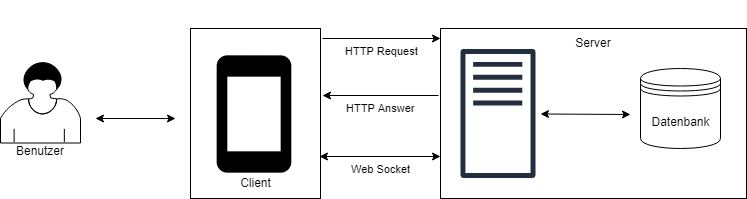
\includegraphics[width=0.8\linewidth]{bilder/server_diagram}
	\caption[Kommunikationsaufbau des zu entwickelnden Systems]{Kommunikationsaufbau des zu entwickelnden Systems}
	\label{fig:server_diagram}
\end{figure}


\subsection{Entwurf des Servers}\label{sec:serverkonzept}
Aufbauend auf das Grundlagen und Analysekapitel sollen in diesem Abschnitt die Entwurfsgedanken hinsichtlich der Serverkomponente des Projekts widergespiegelt werden. 
\subsubsection{Laufzeitumgebung: Node.js}\label{sec:nodejs}
Als Laufzeitumgebung und Grundbaustein des Servers soll die JavaScript-Laufzeitumgebung Node.js genutzt werden, da dies zwei wesentliche Vorteile mit sich bringt:
\begin{enumerate}
	\item Node.js nutzt als Paketmanager und Projektverwaltungstool \textbf{NPM} (Node Paket Manager). Mit dieser Software ist der Zugang zu über 350.000 Paketmodulen (Stand 13. Januar 2017) gegeben und diese können das Projekt Modular erweitern. Ebenso können mit NPM grundlegende Start- und Installationsskripte leicht ausgeführt werden. 
	\item Da Node.js eine JavaScript-Laufzeitumgebung ist, wird zur Programmierung die Skriptsprache JavaScript genutzt, welche auch auf der Clientseite im Webbrowser zum Einsatz kommt. Dies erleichtert den Implementierungsprozess, da einheitlich in einer Sprache geschrieben wird.
\end{enumerate}
Darüber hinaus können NPM-Pakete auch auf der Clientseite genutzt werden (siehe dazu auch Abschnitt \ref{sec:browserify}). Eine gute Skalierbarkeit ist ebenfalls gegeben. Dies wird in folgenden Abschnitten genauer erläutert. Ist ein besonders hohen Ressourcenbedarf von Nöten (z.B. eine Bildungseinrichtung möchte einen zentralen Server installieren, welche viele Klassen/Kurse bedienen soll) können mehrere Serverinstanzen auf einer Maschine parallel laufen und vorab mit einem Lastenverteiler (Load Balancer) Server, wie z.B. NGINX verwaltet werden. Durch die genannte Argumentation soll das Projekt mit NodeJS realisiert werden und nicht mit einem php-Framework. \\ Da Node.js grundlegend sehr offen ist was seinen Einsatzzweck betrifft, soll als Webserver Modul das Node-Paket \textbf{Express.js} genutzt werden, welches im nächsten Abschnitt genauer erläutert wird.
\subsubsection{Webserver: Express}\label{sec:expressjs}
Um mit Node.js komfortabel eine Webapplikation zu implementieren, soll das bekannte Web-Framework Express eingesetzt werden, welches viele HTTP-Dienstprogrammmethoden und den Einsatz von Middlerwarefunktionen gestattet. Hierbei wird jeder eingehende HTTP Request von Funktion zu Funktion weitergeleitet (Aufruf der Methode \texttt{next()}) oder explizit beantwortet (Die Funktion besitzt ein Rückgabewert). Ebenso ist mit Express das Abbilden von Routen möglich. Express soll für den gesamten administrative Teil des Lehrer-Login zum Einsatz kommen. Ebenso soll durch Express das Anlegen und Editieren von Lehreinheiten möglich sein (vgl. \ref{sec:sysbeschreib}). 
Da für den gesamten Lehrer-Backendbereich Express zum Einsatz kommen soll und hier mit einfachen HTTP-Requests gearbeitet wird, kann auf der Einsatz von JavaScript auf der Client-Seite auf ein Minimum reduziert werden, was den Einsatz auf Servereinheiten mit nicht modernem Webbrowser entgegenkommt (Sollte Client und Server auf der gleichen Maschine ausgeführt werden).\\ \\ 
Für den interaktiven Part des Projekts sollen zur Kommunikation WebSockets genutzt werden, welche mithilfe der JavaScript-Bibliothek \textbf{Socket.IO} realisiert werden sollen. Dies wird in der nächsten Sektion beschrieben.   

\subsubsection{SocketIO}\label{sec:socketio}
Die JavaScript-Bibliothek Socket.IO ermöglicht bidirektionale Echtzeit-Kommunikation zwischen Webclient und Server, wobei dabei Bibliothek sowohl auf Server- wie auch Clientseite zum Einsatz kommt. Ein großer Vorteil ist, dass beide Komponenten eine nahezu identische API aufweisen. Daten können sehr einfach von Client ereignisgetrieben (event-driven) zwischen Server und Client sowie vice versa ausgetauscht werden. Client und Server lauschen dabei gegenseitig auf Ereignisse, wie das Verbinden eines neuen Clients oder auch selbst implementierte Ereignisse. Dabei können jegliche JavaScript Daten hin-und hergeschickt werden. Eine händische Konvertierung in das JSON-Format ist nicht notwendig. Für das Anmelden von Schülerinnen und Schülern, das Durchführen von interaktiven Unterrichtsmethoden soll SocketIO zum Einsatz kommen. Hierzu soll Express die entsprechenden Client Daten auf einer festgelegten Route senden und anschließend die Kommunikation von SocketIO kontrolliert werden. Da die Nutzung der Software rein im Intranet nutzbar ist und Nutzende über ein WLAN Zugriff erhalten können, ist der im Abschnitt \ref{sec:websockets} genannte Nachteil von erhöhtem Datenverkehr zu vernachlässigen.      
\subsubsection{Sonstige Module}
Neben Express ist der Einsatz von weiteren Modulen (Node Packages) vorgesehen, welche unterschiedliche Funktionalitäten realisieren sollen. Diese sind:
\begin{itemize}
	\item \textbf{Body-Parser}: Diese Modul ermöglicht das einfach Auslesen von HTTP-Requests möglich. Schickt ein Client bspw. Formulardaten können diese einfach gelesen und ausgewertet werden. Dies soll im Backendbereich der Lehrenden oftmals die Praxis sein.
	\item \textbf{express-session}: Da Lehrende und Administratoren zur Nutzung der Software einen gültigen Zugang besitzen müssen, ist zur Authentifizierung des Nutzenden der Einsatz von Sessions vorgesehen (Querverweis Abschnitt\ref{sec:www}). Das Modul Express-Session macht das Arbeiten mit diesen sehr komfortabel. Über das Zusatzmodul \texttt{connect-session-sequelize} ist die Zusammenarbeit mit der gewählten Datenbank einfach. (Weiterführende Informationen diesbezüglich im Abschnitt  \hyperref[sec:datenbank]{Wahl der Datenbank}). 
	\item \textbf{Pug}: Die Template Engine Pug besitzt seine eigene Syntax und macht das Entwerfen und Schreiben von HTML Templates, welche serverseitig übermittelt werden, sehr komfortabel. Zusätzlich werden Funktionalitäten wie Vererbung und Mixins unterstützt. Ein Einsatzbeschreibung erfolgt in Kapitel \hyperref[sec:implementierung]{Implementierung}. Pug soll für sämtliche zu übertragende HTML Dokumente zum Einsatz kommen.   
\end{itemize}
\subsubsection{Wahl der Datenbank}\label{sec:datenbank}
Da bei dem zu entwickelnden System vielerlei Daten anfallen, wie registrierte Nutzer, angelegte Kurse, interaktive Unterrichtseinheiten und mehr, ist der Einsatz eines Datenbanksystems unerlässlich. Grundlegen können Datenbanksysteme in zwei Kategorien unterteilt werden: \\
\textbf{SQL} und \textbf{noSQL} Systeme. \\ SQL Systeme speichern ihren Daten in sogenannten Relationsmodellen, welche als Tabelle visualisiert werden können. Hierbei beschreibt der Tabellenkopf den Datensatz und seine Datentypus (jede Spalte für sich) während Zeilen eine Entität (Eintrag) in der Datenbank beschreiben. Vorteil hierbei ist, dass die Daten konform sind, d.h. bei Zugriff liefert immer einen Rückgabewert \cite{neumann2015entwicklung}. Nachteil ist der erhöhte Aufwand, sollte die Definition des Relationsmodells im Nachhinein geändert werden, was das Aktualisieren sämtlicher Daten erfordern würde. Desweiteren sind SQL System schwer skalierbar, da für größere Datenbanksysteme potentere Server gekauft werden müssen. Mehrere Relationsmodelle können über Fremd-Schlüsse (Querverweise) miteinander verbunden werden, um auch komplexere Sachverhalte abbilden zu können. \\ \\ NoSQL lassen sich in verschiedene Subkategorien je nach Arbeitsweise beim Speichern der Datensätze einteilen\cite{neumann2015entwicklung}. Am populärsten sind Dokumentenorientiert, Key-Value Pairs (Schlüssel-Wert Paare) und Graphen-basierte Systeme. Dokumentenorientierte NoSQL Datenbanken legen pro Entität ein Dokument an, in welchem die Informationen meist im JSON Format abgespeichert werden. Key-Value Systeme verfolgen ein einfaches Zuordnungsprinzip und bilden Schlüssel-Wert Paare, ähnlich einer Dictionary Datenstruktur. Bei Graphen-basierten Systemen werden Entitäten und ihre Beziehungen untereinander an sich gespeichert. Generell sind NoSQL Systeme weniger statisch definiert im Vergleich zu SQL Systemen. Dies räumt eine große Flexibilität beim Speichern von Daten ein, da Datensätze auch unvollständig gespeichert werden müssen. Dies kann auch als Nachteil interpretiert werden, ist aber generell immer vom Kontext des Projekts abhängig. \\ \\    

Für das zu entwickelnde System soll ein möglichst flexibler Weg gewählt werden was die Wahl der Datenbank betrifft. Da das MVC-Prinzip zum Einsatz kommen soll, beschreibt der Modell Teil von zu bereitstellenden Daten auch wie diese über welche Funktionalität aus der Datenbank geladen werden sollen. Den Controller soll nur die vom Modell bereitgestellten Funktionalitäten nutzen und keine direkten Datenbankzugriffe selbst ausführen. Damit die Software im hohem Maße skalierbar bleibt, ist der Einsatz eines sogenannter Object-Relationship-Mapper, kurz ORM, (Objektrelationale Abbildung) vorgesehen, der an verschiedenste Datenbanksysteme angebunden werden kann. Da das Projekt in seiner kleinsten Skalierung lokal auf einem Einplantinencomputer wie dem Raspberry Pi 3 und im lokal im Intranet laufen können soll, ist für den Anfang die Verwendung eines Datenbanksystems, welches vollständig durch eine Programmbibliothek lauffähig ist, vorgesehen. Dies hat den Vorteil, dass kein extern laufendes Datenbanksystem installiert, gewartet und gestartet werden muss, da die komplette Datenbank in einer einzigen Datei auf dem Server gespeichert wird. Diese Anforderungen erfüllt die gemeinfreie Programmbibliothek \textbf{SQLite}. Die gesamte Datenbank kann hier sogar rein im Arbeitsspeicher gehalten werden, was jedoch den Nachteil mit sich bringt, dass bei einem Ausfall oder Abschalten des Server der kompletten Verlust sämtlicher Daten mit einhergeht. 
\\ Als ORM fiel die Wahl auf das Node.js Modul Sequelize, welches neben SQLite mit viele andere bekannte SQL Datenbanksystemen zusammenarbeiten kann, u.A. Postgres, MariaDB und Microsoft SQL Server. Der Wechsel auf ein anderes SQL Datenbanksystem ist somit jederzeit problemlos möglich, falls gewünscht. \\ \\  

Das Zusatzmodule \texttt{connect-session-sequelize} ermöglicht eine einfache Handhabung der Session-Verwaltung von eingeloggten Lehrenden in das System. Dazu werden entsprechende Tabellen zur Verwaltung der Sessions und deren Lebenszeit automatisch in der Datenbank  via Sequelize angelegt. Zuvor sollen die Passwörter sicher gespeichert werden, d.h. nicht im Klar-Text, nur als Hashwerte welche zusätzlich mit einem Salt verstärkt werden\footnote{Weiterführende Informationen unter:  \url{https://de.wikipedia.org/wiki/Salt_(Kryptologie)}}.

Da zum Zeitpunkt der Recherche kein zu SQLite ähnliches und für den produktiven Einsatz bereites NoSQL Äquivalent gefunden werden konnte, fiel die Wahl auf SQLite. Die genannten Vorteile eines NoSQL Systems scheinen für die Anforderungen des zu entwickelenden Systems ohnehin nicht relevant, obgleich sogar ein Umstieg auf NoSQL Datenbkansystem möglich wäre, auch wenn dies mit einem etwas erhöhten Aufwand einhergeht, da dann auch der ORM gewechselt und die Modelle entsprechend angepasst werden müssten.  

\subsubsection{Server Architekturdiagramm}\label{sec:serverarchitekt}
Schlussfolgernd lässt sich der finale Entwurf des Servers folgend visualisieren und wird in Kapitel \textbf{\ref{sec:implementierung} Implementierung} umgesetzt.

\begin{figure}[H]
	\centering
	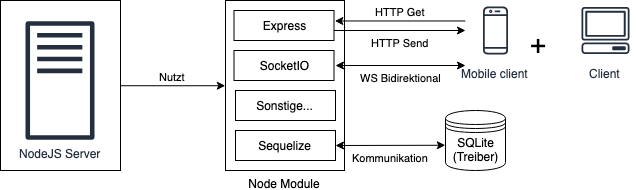
\includegraphics[width=0.8\linewidth]{bilder/server_architektur}
	\caption[Aufbau der geplanten Serverarchitektur]{Aufbau der geplanten Serverarchitektur}
	\label{fig:server_diagram}
\end{figure}
\footnotesize \underline{Hinweis:} NodeJS Module aus der Sektion \textbf{Sonstige Module} wurden aus Gründen der Visualisierung in dieser Grafik nicht näher betrachtet.

\normalsize 
\subsection{Entwurf des Clients}\label{sec:clientkonzept}
Wie zuvor erörtert, ist es vorgesehen drei verschiedene Clients zu implementieren, welche alle auf dem gleichen Prototyp basieren sollen, allerdings verschiedene Zwecke verfolgen. Dies sieht ein Webclient jeweils für \textbf{Lehrende/Dozierende}, \textbf{Schülerinnen und Schüler} und einen für \textbf{Großbildanzeigen} optimierten wie Projektoren o.Ä. vor. Zur Vereinfachung werden diese gemäß der vorherigen Reihenfolge \textbf{Teacher Client}, \textbf{Student Client} und \textbf{Presenter Client} in diesem und darauffolgendem Kapitel genannt.\\ \\ 

\subsubsection{Gedanken zu UI}\label{sec:uientwurf}
Da das Projekt als Web-Applikation implementiert werden soll, wird die UI gänzlich durch die Stylesheet-Sprache CSS beschrieben. Im Jahr 2018 wurden erstmals häufiger mobile Endgeräte wie Smartphones zur Internetnutzung herangezogen als der klassische Computer oder Laptop\cite{Rabe2019}. Viele Design-Frameworks setzen daher schon länger auf das Prinzip 'Mobile First'. Da die Applikation letztlich sowohl auf Computern und Smartphones aber auch Großbildgeräten angezeigt werden soll, bildet ein flexibles Web-Design-Framework als Basis, welches bereits viele relevante Web-Design Standards wie das o.g. 'Mobile First' berücksichtigt, ein solides Fundament in Sachen Usability und Design. Eines der populärsten dieser Art ist \textbf{Bootstrap}, welches zusammen mit einem frei erhältlichen Design-Theme von \url{https://freehtml5.co/} genutzt werden soll. Das gewählte Theme soll an die Applikation angepasst und teils für die Großbild Anzeige des Presenter Clients optimiert werden.  
\subsubsection{Browserify}\label{sec:browserify}
Um das Nutzen von Node.js Packages sowie damit verbundene \texttt{require()} Funktionalität auch auf der Clientseite zu ermöglichen, soll die JavaScript Bibliothek \textbf{Browserify} zum Einsatz kommen. Mit ihr können alle Node.js Packages, welche über den Node Package Manager in das Projekt hinzugefügt wurde im Webbrowser des Clients genutzt werden. Dazu bündelt die Bibliothek alle Module und stellt anschließend eine einzige JavaScript Datei zur Verfügung, die nur noch im HTML-Dokument eingebunden werden muss. Mithilfe der \texttt{require()} Funktionalität, welche von Node.js gestellt wird, kann der Code auch übersichtlicher in mehrere Dateien/Module aufgeteilt werden. Dies war ohne Aufwand auf der Browserseite nicht ohne weiteres möglich, ist aber durch die Einführung von Modulen seit ECMAScript\footnote{Der als ECMAScript (ECMA 262) standardisierte Sprachkern von JavaScript beschreibt eine dynamisch typisierte, objektorientierte, aber klassenlose Skriptsprache. (Wikipedia.org)} in Version 6  nun möglich. Oftmals wird aber aus Kompatibliltätsgründen  zu älteren Webbrowsern auf Lösungen wie Browserify oder auch Babel gesetzt. Letztere übersetzt den geschriebenen JavaScript Code so, dass er auch von älteren Webbrowsern interpretiert wird (auch Transpiler genannt). Sämtliche folglich genannten JavaScript Module resp. Bibliotheken sollen via Browserify in eine JavaScript Datei zusammengefasst werden und anschließend pro Client eingebunden werden. Das bringt den zusätzlichen Vorteil dass für jegliches, auf Browserseite eingesetztes JavaScript nur einen einzigen HTTP-Get Request benötigt, da wie erwähnt nur eine JavaScript Datei pro Client angefordert werden muss. 
\subsubsection{JavaScript Lösungen}\label{sec:clientjs}
Von folgenden JavaScript Lösungen soll auf der Clientseite Gebrauch gemacht werden, um den Implementierungsprozess zu optimieren:
\begin{itemize}
	\item \textbf{VueJS}: Um das Anzeige, Editieren und Anpassen dynamischer Inhalte zu erleichtern, soll das JavaScript-Webframework VueJS zum Einsatz kommen, da dieses gut skalierbar ist und alle benötigten Funktionalitäten mit sich bringt. Im Vergleich zu AngularJS und React (siehe auch Abschnitt \ref{sec:clientseitigeransatz}), biete VueJS eine flachere Lernkurve und kann als ein guter Kompromiss aus seinen zwei Konkurrenten betrachtet werden. Mittlerweile hat VueJS seinen Konkurrent React in Sachen Popularität auf GitHub überholt\cite{Daityari2019}. VueJS ist auch gemessen an der Dateigröße von nur 80 KB deutlich kleiner im Vergleich zu Angular mit 500 KB.
	\item \textbf{SocketIO}: Das bereits in Abschnitt \ref{sec:socketio} erwähnte SocketIO besitzt ein Gegenstück, welches auf der Clientseite im Webbrowser zum Einsatz kommt. Dadurch wird die bidirektionale Kommunikation mit der Server ermöglicht und es soll in beide Richtungen Daten in Echtzeit ausgetauscht werden. 
	\item \textbf{Zingchart}: Zur Visualisierung der Wörterwolke (WordCloud), welche bei der interaktiven Unterrichtsmethode Brainstorming zum Einsatz kommt, und sonstigen Diagrammen soll die auf diese Szenarien spezialisierte JavaScript Bibliothek ZingChart genutzt werden. Die Software ist in einer freien Version erhältlich, wobei lediglich ein kleines ZingChart Logo stets angezeigt werden muss\cite{zingchartpricing}.
\end{itemize}

\subsubsection{Client Architekturdiagramm}\label{sec:serverarchitekt}
Nachfolgend die umzusetzende Architektur der Client-Anwendung. 

\begin{figure}[H]
	\centering
	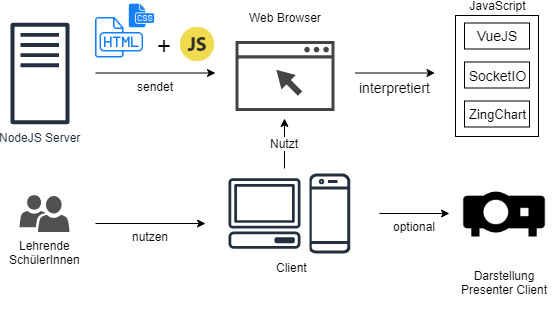
\includegraphics[width=0.8\linewidth]{bilder/client_architektur}
	\caption[Aufbau der geplanten Client Architektur]{Aufbau der geplanten Client Architektur}
	\label{fig:client_diagram}
\end{figure}
\footnotesize \underline{Hinweis:} Zum besseren Verständnis wurden die Rollen des Servers und der Nutzer ebenso dargestellt. Der Presenter Client nutzt in der Grafik ein Projektor. Dies ist eine Option und nicht zwingend von Nöten. Alle Clients können auf der gleichen Maschine ausgeführt werden (z.B. in unterschiedlichen Tabs eine Webbrowsers) als auch auf entfernten. 

\normalsize

\newpage

\section{Implementierung}\label{sec:implementierung}
%TOTO LEFTOVER: 
%QUIZ
%HTTPS
%WLAN
Das folgende Kapitel wird Einblicke in die Entwicklung der Software im Rahmen des Projekts geben. 
Dabei wird iterativ chronologisch die Vorgehensweise schriftlich reflektiert und an mehreren Stellen 
zum besseren Verständnis auch ein Einblicke in den Sourcecode gegeben. Anknüpfend werden etwaige Probleme bei der Implementierung aufgezeigt sowie mögliche Lösungen diskutiert. 

\subsubsection{Implementierung der Server-Software}\label{sec:implementserver}
Aufbauend auf das Entwurf Kapitel soll die Server-Software mit NodeJS und ExpressJS als Hauptkomponente entwickelt werden. Dazu wird zunächst im folgenden Abschnitt \ref{sec:implementexpress} der HTTP Server grundlegend konfiguriert und anschließend dessen Routen im darauffolgenden Kapitel \ref{sec:anlegrouten} angelegt. 

\subsubsection{ExpressJS Setup}\label{sec:implementexpress}
Nachdem das Projekt grundlegend mit dem Befehl \texttt{npm init} initialisiert wurde,
kann ExpressJS einfach über den Node Packet Manager (nachfolgend NPM genannt) hinzugefügt werden. 
Zusätzlich wird das NPM Paket IP genutzt um die aktuelle IP-Adresse der Maschine zu automatisch ermitteln und
den ExpressJS Server auf dieser lauschen zu lassen. Dies ist mit wenigen Zeilen Code erledigt:
\begin{lstlisting}[caption=Errichtung des Webservers]
const app = express();
const server = app.listen(3000, server_ip, function () {
logger.log({ level: 'info', message: `Hello! The Server is running on ${server_ip}!`});
});
\end{lstlisting}
Der Server lauscht auf der IP Adresse des Adapters der Maschine auf dem er ausgeführt wird, zusätzlich auf Port 3000, dies sollte je nach Konfiguration auf den Standard HTTP Port 80 resp. 443 geändert werden, sollte Verschlüsselung eingerichtet sein (HTTPS).
\\
Anschließend können nun die Routen eingerichtet werden.

\subsubsection{Autarkes WLAN}\label{sec:eigeneswlan}
Um einen Stand-Alone Betrieb\footnote{Stand-Alone meint einen Betrieb unabhänging von ggf. vorhandenen Netzwerkinfrastruktur am Einsatzort} der Software zu ermöglichen, wird als Lösung der Betrieb eines unabhängigen kabellosen Netzwerkes (WLAN/Wifi) angestrebt. Folgende mögliche Lösungsszenarien wurden ausgearbeitet.
\begin{enumerate}
	\item \textbf{Einfach}: Als einfachste Lösung hat sich der Betrieb eines lokalen WLANs über ein Smartphone oder Laptop herausgestellt. Nahezu jedes Smartphone bzw. jeder Laptop lässt das generieren eines WLAN Zugangspunkt für andere Geräte zu. Der Server wird mit diesem Netzwerk verbunden, sowie alle Clients. Dies wurde getestet und ein Betrieb war möglich. Da hierbei aber auch die Internetverbindung des Zugangspunktes freigegeben wird, was ggf. unerwünscht sein kann, würde es sich anbieten eine spezielle 'Companion App' zu entwickeln und für Android / iOS basierte Smartphones zu entwickeln. Diese könnte automatisch einen WLAN-Hotspot erstellen und den Netzwerkverkehr eventuell limitieren. Gleiches gilt analog für windows- oder unixbasierte Computer, ist aber problematischer, siehe dazu nächsten Listenpunkt.
	\item \textbf{Speziell}: Um auf einem Computer vollautomatisch einen WLAN Hotspot zu genieren, bedarf es Administrator Privilegien sowie genauere Kenntnisse über den verwendeten Netzwerkadapter. NodeJS selbst bietet nur eingeschränkt Möglichkeiten an, diese Aufgabe autark zu übernehmen, könnte aber ggf. eventuelle Shell-Skripte triggern. Unter Microsoft Windows 7+ gibt es mit den NPM Paket \texttt{node-hotspot} auch die Möglichkeit, dies direkt mit NodeJS zu erledigen. Diese Paket wird in die zu entwickelnde Software integriert und soll anschließend unter einer Microsoft Windows Umgebung das generieren eines WLAN Hotspots / Zugangspunktes ermöglichen. Zur Verwendung werden entsprechende Steuerungsoptionen in Einstellungsbereich im Lehrkraft Backend integriert. Die interne Steuerung erfolgt über Routen (siehe auch Abschnitt \ref{sec:anlegrouten}).
	
Wird die Applikation in einer vorhandenen Netzwerkinfrastruktur betrieben, ist ein Betrieb in jedem Falle gewährleistet. Ein mobiler WLAN-Router könnte ebenfalls genutzt werden, sollte keine ausreichende Infrastruktur vorhanden sein. Dieser müsste einmalig konfiguriert werden und ist anschließend in der Lage die Serverapplikation für Clients ansprechbar zu machen. Ein solches Gerät gibt es bereits ab ca. 10 Euro zu erwerben.
\end{enumerate} 

\subsubsection{Verschlüsselung}\label{sec:encrypted}
Um eine verschlüsselte Kommunikation zwischen Server und Clients zu gewährleisten, ist der Datenaustausch über das HTTPS Protokoll vorzuziehen. Um HTTPS allerdings sinnvoll nutzen zu können, ist ein Zertifikat von einer Zertifizierungsstelle (CA) notwendig, was meist mit Kosten verbunden ist. Allerdings bietet der Anbieter \textbf{Let's Encrypt}\cite{LetsEncrypt.org} kostenlose Zertifikate an, welche sich problemlos bei vorhandenem SSH-Zugang installieren lassen. Für den Intranet Betrieb können relativ einfach eigens ausgestellte Zertifikate genutzt werden, welche mit Shell-Programmen wie \textbf{openssl} generierbar sind\cite{Copes2018}. Allerdings warnen moderne Webbrowser den Nutzenden recht auffällig, dass die genutzte Verbindung dennoch nicht sicher ist, da dem Zertifikat nicht vertraut werden kann. Der HTTPS Betrieb wurde erfolgreich getestet. Die Implementierung ist nicht aufwendig allerdings, birgt aber den o.g. Nachteil. Da das Intranet ein an sich abgeschlossenes Netzwerk ist, scheint der verschlüsselte Betrieb in diesem zunächst nicht wichtig, kann aber jederzeit realisiert werden und ist bei Betrieb im Internet als obligatorisch zu betrachten. 

\subsubsection{Anlegen der Routen}\label{sec:anlegrouten}

Grundlegend soll es folgende Routen auf dem Server geben:
\begin{itemize}
	\item \textbf{'/'}: Die Haupt Route, sie wird angesteuert, wenn der Server einfach unter seiner IP (oder eingerichteter Domain) kontaktiert wird. Hier wird anschließend die Rolle des Nutzers (Lehrender oder Schülerin/Schüler) abgefragt  und dementsprechend weitergeleitet.
	\item \textbf{'/teacher'}: Diese Route verweist auf den Lehrerbereich der Anwendung, man kann sie auch als Backendbereich bezeichnen. Alle hinter dieser Route liegende Routen bedürfen einer Authentifizierung seitens des Nutzenden.
	\item \textbf{'/client'}: Diese Route verweist grundlegend auf den Student Client. Aber auch der Presenter Client wird über diese Weiche aufgerufen. 
\end{itemize}
Neben diesen drei Hauptrouten existieren noch weitere spezial Routen für das Error-Handling (z.B. 404 - Seite nicht gefunden) sowie besondere für die WebSocket Kommunikation, welche aber im Hintergrund genutzt werden und im Abschnitt \ref{REF UNKNOWN YET!} beleuchtet werden.\\ 
Das Anlege der Routen ist mit folgendem Codeausschnitt durchgeführt:
\begin{lstlisting}[caption=Anlegen der Routen]
app.use('/teacher', teacherRoutes);
app.use('/client', clientRoutes);
app.use('/', mainRoutes);
\end{lstlisting}
\footnotesize{Die Route Module werden im Hauptmodul (app.js) referenziert und deren Zuständigkeit festgelegt.}
\normalsize
Zu beachten gilt: Die weiterführend Routen werden in Dateien ausgelagert, um die Übersicht des Quelltextes zu wahren. Ebenso sind auch diese Routen sog. Middleware-Funktionen. Dies wird im nächsten Abschnitt genauer beleuchtet. Daher ist auch die Reihenfolge wichtig, würde die \texttt{'/'} Route als erstes angelegt werden, so würde diese alle folgenden, spezifischeren 'abfangen'.  


\subsubsection{Reflexion des MVC Schemas}\label{sec:mvc}
Da der Server nach dem Model-View-Controller Muster grundlegend arbeiten soll, gilt es dieses zu implementieren. Die folgende Tabelle soll ein Überblick über die anfallende Struktur geben:

\begin{table}[h!]
	\caption{MVC Struktur der Implementierung}
	\label{tab:mvcschema}
	\begin{tabular}{|l|l|l|l|}
		\hline
		\multicolumn{1}{|c|}{\textbf{Betrifft}}                         & \multicolumn{1}{c|}{\textbf{Model}} & \multicolumn{1}{c|}{\textbf{View(s)}}                                                                         & \multicolumn{1}{c|}{\textbf{Controller}}                                            \\ \hline
		Lehrende                                                        & user.js                             & \begin{tabular}[c]{@{}l@{}}teacher/new.pug\\ teacher/signup.pug\\ teacher/user-edit.pug\end{tabular}          & teacher.js                                                                          \\ \hline
		\begin{tabular}[c]{@{}l@{}}Schülerinnen/\\ Schüler\end{tabular} & student.js                          & student.pug                                                                                                   & client.js                                                                           \\ \hline
		Lehreinheiten                                                   & eduSession.js                       & \begin{tabular}[c]{@{}l@{}}edusessions/*/*.pug\\ edusessions/index.pug\\ edusessions/running.pug\end{tabular} & \begin{tabular}[c]{@{}l@{}}session.js\\ quizzing.js\\ brainstorming.js\end{tabular} \\ \hline
	\end{tabular}
\footnotesize {
	Zum Zwecke der Übersicht wurden einige interne Controller-Dateien nicht gelistet, wie z.B. der Error-Controller, welcher zwar eine View besitzt, jedoch kein Model. 
}
\end{table}
\newpage
Folglich müssen die entsprechenden Controller-Funktionen an Routen gebunden werden. Dabei wurde sich teils am RESTful Design orientiert, die Umsetzung erhebt jedoch kein Anspruch vollkommen 'RESTful' zu sein. Zunächst müssen entsprechende Unterrouten zu den aus Abschnitt \ref{sec:anlegrouten} bereits angelegten hinzugefügt werden. Zwecks der Übersicht wird hierzu ein Routes Ordner angelegt, welche die entsprechenden Router enthalten soll. 
Folgende Router werden angelegt: \\ \\
\textbf{routes/client.js}: Legt alle Student Client und Presenter Client relevanten Routen fest.\\
\textbf{routes/teacher.js}: Alle für das Backend resp. Lehrerbereich relevanten Routes werden hier angelegt.\\
Es folgt ein Codebeispiel aus der Datei routes/client.js. 
\begin{lstlisting}[caption=Unterrouten und Controlleranbindung]
// 3rd Party Imports
const express = require('express');
const router = express.Router();
// App Imports
const clientController = require('../controllers/client');
const isAuth = require('../middleware/is-auth');
// Presenter & Student Clients
router.get('/presenter/:sessionId', isAuth, clientController.getPresenter);
router.get('/student', clientController.getStudent);
router.get('/', clientController.getStudent);
module.exports = router;
\end{lstlisting}
Zur Verdeutlichung wird anknüpfend die in Zeile 10 des vorangegangen Listings Funktion \texttt{getStudent} des Controllers gezeigt:
\begin{lstlisting}[caption=GET Funktion des Student Controllers]
// GET => /client/student
exports.getStudent = (req, res, next) => {

return res.render('client/student',
	{
		docTitle: 'Student | Node ICT',
		ipAdd: ip.address(),
	});
};
\end{lstlisting}
 
 \subsubsection{Einrichtung der Datenbank}
 Die SQL Datenbank 'SQLite'  und der Object-Relationship-Mapper 'Sequelize' können einfach über den NPM dem Projekt hinzugefügt werden.  
 Nach diesem Schritt kann die Anbindung und Einpflegung folgen. Hierzu wird ein Datenbank Utility Modul angelegt, dieses soll die grundlegende Konfiguration der Datenbank enthalten und ausführen. All dies kann direkt über Sequelize erfolgen, welches im Hintergrund die notwendigen Schritte vornimmt. Es muss der Dialekt 'sqlite' angegeben werden und der Pfad unter welchem die Datenbank als Datei gespeichert werden soll. \\ 
 Gemäß dem logischen Aufbau einer SQL Datenbank folgt nun das Konfigurieren und Anlegen der Tabellen und deren Beziehung untereinander. Dieser Arbeitsschritt erfolgt relativ intuitiv. Im folgenden Code-Beispiel wird die Tabelle bzw. Sequelize Model 'student' im Modul tables konfiguriert.
 
 \begin{lstlisting}[caption=Anlegen einer Tabelle und deren Beziehungen]
exports.student = (sequelize, Sequelize) => {
	return sequelize.define('student', {
		id: {
			type: Sequelize.INTEGER,
			autoIncrement: true,
			allowNull: false,
			primaryKey: true
		},
		name: {
			type: Sequelize.STRING,
			allowNull: false
		},
	})
};
 \end{lstlisting}
 Im Datenbank Utility Modul wird nun die Konfiguration geladen und anschließend dessen Beziehung zu anderen Entitäten eingestellt. Durch Sequelize kann hier ein relativ humanes Sprachbild verwendet werden. Das folgende Beispiel zeigt die Beziehungen zwischen EduSession und Student an:
 \begin{lstlisting}[caption=Konfiguration von Entitätsbeziehungen]
 EduSession.hasMany(Student, { onDelete: 'cascade' });
 Student.belongsTo(EduSession);
 \end{lstlisting}
 Nach dem selben Schema werden nun für alle Modelle entsprechende Tabelle angelegt und deren Beziehungen untereinander festgelegt. 
 \paragraph{Datenbank Interaktion}
 Um Datenbank Anfragen (Queries) zu stellen, bietet Sequelize viele Optionen an. Diese müssen nicht in SQL geschrieben werden, sondern sind normale JavaScript Funktionen. Jedes innerhalb Sequelize definierte Model bietet diese automatisch an. Als Beispiel könnte nun über 
 \texttt{const studentToFind = Student.findByPk(1);} die Entität mit der ID 1 geladen werden. All diese bereitgestellten Funktionen sind JavaScript Promises, d.h. sie werden asynchron ausgeführt und es Bedarf entsprechendes Handeln im Fehlerfall.
 Im Erfolgsfall befindet sich in der Variabel nun das Objekt der Entität und dieses bietet wiederum Funktionen zur Interaktion an. Eine ausführliche Dokumentation findet sich auf der Webpräsenz von Sequelize. 
 Die in Tabelle \ref{tab:mvcschema} gelisteten Modelle werden gemäß der Arbeitsteilung des MVC-Schemas hauptsächlich direkt mit Sequelize arbeiten und den Controllern entsprechende Funktionen bereitstellen.
 \subsubsection{Implementierung des LehrerInnen Bereiches}\label{sec:implementlehrer}
 %hier halt sessions zum einlogge
 % Das Grundsetup wenn alles neu
 % User Anlegen / Freischalte / Sicherheit bei der Datenfreigabe 
 % Anlegen von Lehreinheiten + Brainstorming + Quizzing
 Nachdem die aus Abschnitt \ref{sec:mvc} genannten Model-Module angelegt wurden, welche direkt mit der Datenbank interagieren, müssen anschließend Controller für die verschiedenen Abschnitte des Webservers implementiert werden. Jedes Model hat dabei einen zugehörigen Controller, welcher entsprechende Funktionen für die Routen exportieren soll. Wie in Listing 3 beispielhaft zu sehen, wird die GET-Route '/student' mit der nach außen hin exportierten Funktion \texttt{getStudent} assoziiert. Um eine einheitliche Struktur zu gewährleisten, werden exportierte Funktionen eines Controller Moduls immer nach der jeweilig bedienten Request-Methode benannten (GET, POST, etc.). \\
 \paragraph{View Rendering mit PUG}
Für alle Views soll die Template Engine Pug zum Einsatz kommen (siehe auch Kapitel \ref{sec:konzept} Konzept). Dazu wird PUG für das Rendern aller nicht statischen Routen im Hauptmodul der Software registriert. PUG macht das Schreiben von HTML Dokumenten sehr komfortable und unterstützt Vererbung (Layouting). So wird zunächst für den LehrerInnen Bereich ein Main Layout angelegt, von dem später alle anderen, diesem Bereich zugehörigen, Views erben. Die Layouts können zusätzlich so genannte Blöcke enthalten, welche später dann dynamisch mit Inhalten von Views gefüllt werden, welche vom Main Layout erben. Die Controller können Daten an die Views übergeben, welche von diesen dann dargestellt werden. Dazu bietet PUG wie die meisten Template Engines Funktionen an, wie das Iterieren über Datensätze mittels Schleifen ermöglicht oder dynamisch generierte Inhalte abhängig von konditionalen Ausdrücken. Sämtliche an die Clients ausgelieferte HTML Dokumente sollen von PUG on-demand generiert werden. PUG benutzt seine eigene Templating-Language, welche sich deutlich von dem bekannten HTML unterscheidet, aber sehr intuitiv und schnell zu lernen ist. So wird die Hierarchie der HTML Elemente allein durch Einrückung bestimmt. Somit entfällt das Schließen dieser komplett. \\ 
Es werden anschließen für alle Modelle Views angelegt, damit Lehrende sich anmelden und einloggen sowie neue Benutzer anlegen und editieren können. Ebenso für das erstellen von Lehreinheiten vom Typ Brainstorming und Quiz. Dabei werden bei Dateneingabe seitens der Nutzende Formulare verwendet, welche anschließend via POST Request an den Server geschickt und dort von Controllern und ihren jeweiligen Modellen ausgewertet. Das tatsächliche Ausführen und dessen Entwicklung wird im später folgenden Abschnitt \textbf{\ref{sec:implementsessions} Implementierung der Lehreinheiten} beschrieben. 
\\ 
HIER NOCH EIN LISTING?
\paragraph{UI Design}
Aufbauend auf den Abschnitt \ref{sec:uientwurf} des Entwurf-Kapitels wird zur Designumsetzung das Frontend-CSS-Webframework \textbf{Bootstrap} genutzt. Dieses kann ebenfalls einfach über NPM dem Projekt hinzugefügt werden. Als Design-Theme soll das frei erhältliche Bootstrap Theme \texttt{Neat} von \textbf{freehtml5.co} die Grundlage bilden. Dieses wird gänzlich im Backend-Bereich des Lehrkraftzugangs genutzt, angepasste Teile anknüpfend für den Student Client und den Presenter Client, welche insbesondere noch durch eigenen CSS Code für die Nutzung auf Großbildgeräten wie Fernsehern und Projektoren optimiert wird. Es wird sichergestellt dass sich die Software angenehm auf stationären wie mobilen Endgeräten nutzen lässt. 

\begin{figure}[h!]
	\centering
	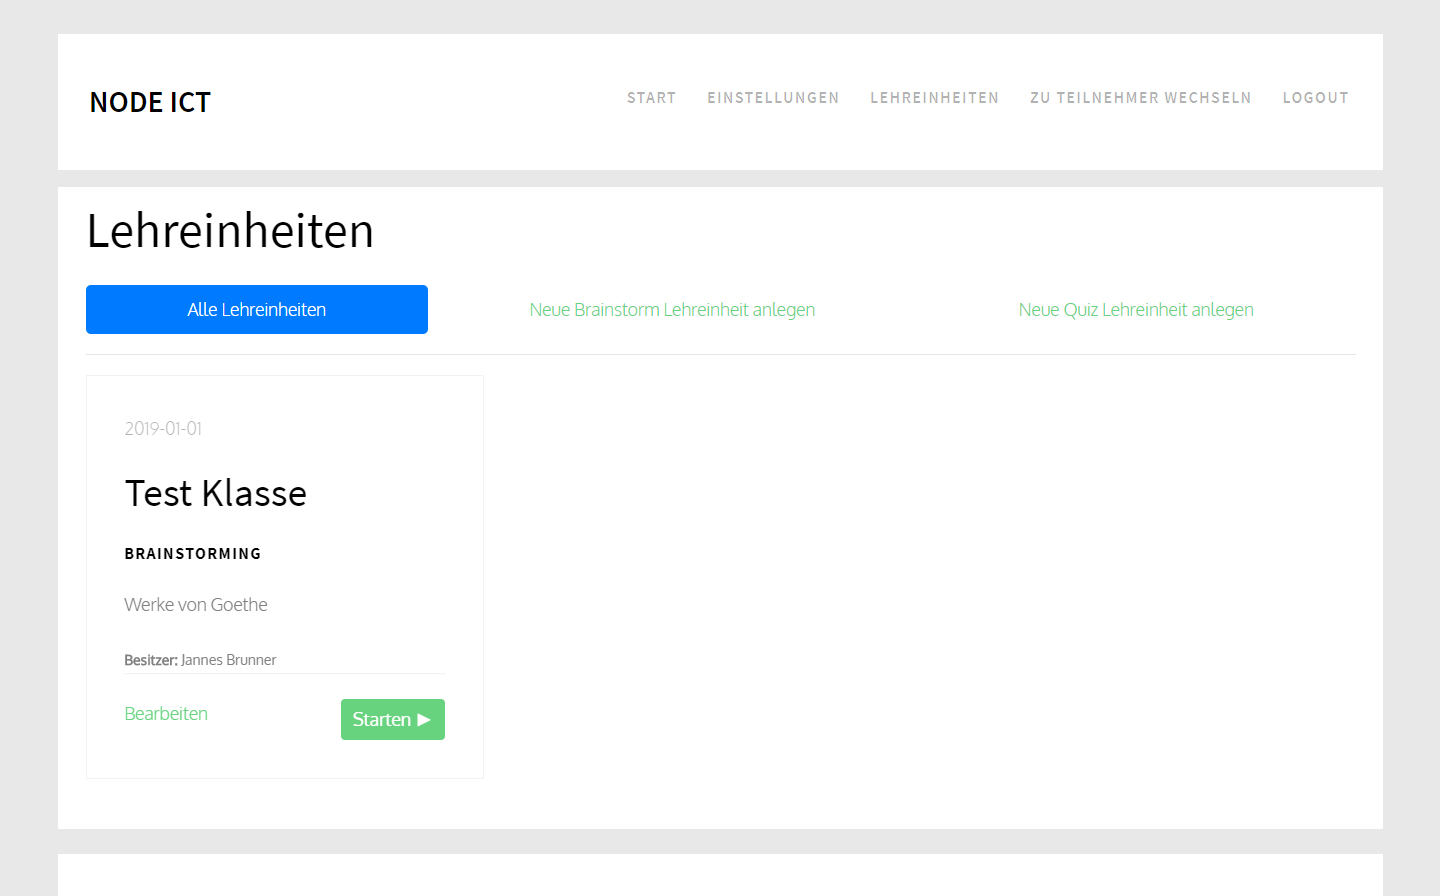
\includegraphics[width=0.9\linewidth]{bilder/screenshot_lehreinheiten}
	\caption[Screenshot UI Design Lehreinheitenbereich]{UI Design der Applikation beispielhaft illustriert durch ein Screenshot des Lehreinheiten Bereiches im Backend Zugang des Teacher Clients.}
	\label{fig:screenshot_lehreinheiten}
\end{figure}

\paragraph{Absicherung des Bereiches}
Bestimmte Bereiche der Applikation sollen nur registrierten und freigeschalteten Benutzenden zugänglich sein. Beim erstmaligen Initialisieren wird der Server mit einem Super-Administrator Account eingerichtet. Nur dieser soll neue Nutzer freischalten, andere Lehrende zu Administratoren ernennen und die Applikation auf Werkseinstellungen zurücksetzen können. Eine entsprechende Einrichtungsmaske soll beim ersten Serverstart automatisch erscheinen. Um dies technisch zu realisieren, wird das aus dem \textbf{Konzept} Kapitel genannte \texttt{express-session} NPM-Modul genutzt, welches bereits vollständig mit der von Sequelize verwalteten SQLite Datenbank einsatzbereit ist. Nach der Einrichtung im Hauptmodul wird eine eigene Middleware geschrieben, welche bei allen abgesicherten Routen als erstes aufgerufen wird und überprüft, ob die vom Client übertragene Session noch gültig ist.
\begin{lstlisting}[caption=Code der Authentifizierungs Middleware]
module.exports = (req, res, next) => {
	if(!req.session.isLoggedIn) return res.redirect('/teacher/login');
	next();
}
\end{lstlisting}
Falls dies nicht Fall ist, wird auf die Login Seite verwiesen. 
Das Verwalten der Sessions und das generieren von Cookies für die Client-Seite wird automatisch von dem Modul übernommen.
 \subsubsection{Umsetzung des Client Softwareanteile}\label{sec:implementclients}
 %Hier auch setup, browserify! 
 % vuejs, etc pp
Nachdem die Funktionalitäten Erste Initialisierung der Software, Login/Logout und Benutzerverwaltung sowie das Anlegen und Verwalten von Lehreinheiten des Typs Brainstorming und Quiz implementiert sind, sollen die Lehreinheiten auch aktiv ausgeführt werden können. Dies bildet die Hauptfunktionalität der Software und verlangt mehr Interaktion auf der Client Seite.\\ \\ Die \textbf{Browserify} Software wird einfach über den NPM der Projekt hinzugefügt und ist sofort einsatzbereit. Alle im Abschnitt \ref{sec:clientjs} des Konzeptkapitels erwähnten JavaScript Lösungen sind als NPM Packet verfügbar und werden ebenfalls dem Projekt hinzugefügt. Pro Client (Teacher Client, Student Client, Presenter Client) wird ein Development-Modul angelegt. In diesem können alle benötigten JavaScript Bibliotheken normal importiert und genutzt werden. 
Via Browserify wird anschließend pro Client ein Production Modul generiert, welches alle notwendigen Importe bündelt. Um diesen Prozess zu automatisieren, wird ein Skript erstellt, welches vom NPM ausgeführt werden kann. Nur das Production Modul muss via \texttt{script} Tag in das jeweilige Pug Template pro Client eingebunden werden. Dies reduziert gleichzeitig die Anzahl notwendiger GET-Requests auf der Client-Seite. \\
Pro Client wird die UI mit dem JavaScript Framework \textbf{Vue.js} kontrolliert und verwaltet. 
Auf dem HTML Layout wird ein \texttt{div} Element als Ankerpunkt definiert und alle unterliegenden Elemente stehen fortan zur dynamischen Anpassung bereit. Mittels Datenbindung (Data-Binding) hält VueJS die angezeigten Informationen auf dem UI aktuell. VueJS ist dabei pro Client als einfaches JavaScript Objekt auch von außen ansprechbar, was die Schnittstelle für andere Bibliotheken, insbesondere SocketIO, bildet. \textbf{SocketIO} auf der Client-Seite ist für den gesamten Datenverkehr zwischen Server und Client verantwortlich. Sowohl auf Server- wie auch Client-Seite können Listener programmiert werden, die auf bestimmte Ereignisse (Events)  von der jeweils anderen Seite ausgelöst, lauschen. Im Ereignisfall wird eine anonyme Funktion aufgerufen, welche sich um die eintreffende Daten kümmert. Die ausgetauschten Daten müssen hierbei nicht zwangsläufig zuvor indas  JSON-Format umgewandelt werden, wie dies sonst bei REST-Apis üblich ist. \\ Auf der Server-Seite kümmert sich das Modul \texttt{ioSocketHandler} um alle eingehend Web-Socket Verbindungen und ordnet diesen zunächst einem Namensraum (Namespace) zu. Ein Student Client wird dabei immer dem Namensraum für Student Clients zugeordnet und steht als Socket Objekt zur Verfügung, übliche Clients diesem Schema folgend.  Nach erfolgreicher Verbindung wird dem Student Client eine Liste verfügbarer Lehreinheiten geschickt und diesem auf der Client Seite dargestellt. Pro Lehreinheittyp (Brainstorming und Quiz) gibt es einen  'Session Handler', der als JavaScript Klasse implementiert ist. Startet eine Lehrkraft eine Lehreinheit wird abhängig vom Typ eine neuen Klasseninstanz angelegt und eine Referenz gehalten. Tritt nun eine Schülerin oder ein Schüler der Lehreinheit bei, übergibt das übergeordnete 'Socket Handler'-Modul das Socket-Objekt der Klasseninstanz der Lehreinheit. Die gesamte Logik und Kommunikation der auszuführenden Lehreinheit (Session) wird von der jeweiligen Klasse übernommen. Beendet eine Lehrkraft die Session, wird diese aus dem Speicher entfernt und steht nicht mehr zum beitreten zur Verfügung. Pro gestartete Session kann über einen speziellen Link der passende Presenter Client aufgerufen werden. Dieser wird ebenfalls über das \texttt{ioSocketHandler} Modul der jeweiligen Lehreinheiten Klasseninstanz zugeordnet. Es folgt ein Codeauszug welcher den Datenaustausch zwischen Server und Client zeigt.
\begin{lstlisting}[caption=Server Socket Event Emitierung]
/// TEACHER :::::::
updateSessionT() {
	this.socketT.emit("updateSession", this.session);
}
\end{lstlisting}
\footnotesize
Der Server schickt das Event 'updateSession' an den Teacher Client.
Als Inhalt der Nachricht wird das Session Objekt ('this.session') übermittelt.
\begin{lstlisting}[caption=Client Socket Event Listener]
// Sever tells client to update the session object
socket.on("updateSession", function (newSession) {
	console.log("getting fresh session from server...", newSession)
	if (newSession && newSession.id == vue.session.id) {
		vue.session = newSession;
	}});
\end{lstlisting}
\footnotesize
Der Teacher Client lauscht auf das Event 'updateSession'. Trifft dieses ein,
wird eine anonyme Funktion aufgerufen, welche sich dem Inhalt der Nachricht annimmt.
Diese überprüft in diesem Fall zunächst, ob sich die ID des zu aktualisierenden Session Objekts
mit dem ursprünglichen deckt. Anschließend wird das alte Session Objekt auf das neue referenziert. 

\normalsize 
 
\subsubsection{Problemstellen der Implementierung}\label{sec:probsserver}
%ioSessionHandler Socket Handling
%Word Cloud passende finden und praktikabel 
%Wifi Hotspot node module 
%Allgemeiner Umfang von VueJS und sein Einsatz
Während der Implementierung stellte sich anfangs das Verbindungsmanagement der verbundenen Clients über SocketIO als instabil heraus, da Sockets bei jedem Verbindungsabbruch sich zwar selbständig erneut verbinden, jedoch immer unter einer neuen Session ID. Dies führte zunächst zu unerwartetem Verhalten während einer ausgeführten Lehreinheiten Ausführung. Dem konnte aber durch zusätzliche Authentifizierungsdaten entgegengewirkt werden. Bei mobilen Geräten wie Smartphones scheint dies auch geräteabhängig zu sein, da manche hier die Verbindung z.B. beim Ausschalten des Bildschirms sofort unterbrechen, während andere diese im Hintergrund weiter aufrecht erhalten. \\ Ebenso war es schwierig ein gut funktionales Word-Cloud / Wörterwolke Modul zu finden, welches sich ohne nennenswerte Probleme mit VueJS im Einklang nutzen lassen konnte. Generell wird VueJS in diesem Projekt recht rudimentär eingesetzt, was seine Funktionsweise zwar nicht einschränkt, jedoch das volle Potential dieser Web-Frontend-Engine nicht gänzlich nutzt. Eine tiefgreifendere Einarbeitung in VueJS ist aus Zeitmanagement Gründen nicht erfolgt. \\ \\ Das NPM-Modul \texttt{node-hotspot} wurde zwar gemäß der Instruktionen der Entwickler implementiert, allerdings konnte auf mehreren Microsoft Windows Testsystemen nicht selbstständig ein WLAN-Hotspot aktiviert werden. Alternative Module erwiesen sich als ungenügend. 
 
 
 
\newpage

\section{Erprobung}\label{sec:erprobung}
\newpage

\section{Auswertung}\label{sec:auswertung}
\newpage

\section{Ausblick}\label{sec:ausblick}
%electron!
%  Eine hier angesetzte Refaktorierung ist vuejs und socketIO
% REST statt Sockets
% 
\subsection{Optimierungspunkte der Software}\label{sec:opti}
Der Nachrichtenaustausch, welcher über das \emph{WebSocket} Protokoll via \emph{Socket.IO} realisiert ist, sollte mehr vereinheitlicht werden. Grundsätzlich lassen sich jede Art von \emph{JavaScript} Daten übertragen; ein strengeres Konzept kann hier das Verständnis für andere Entwickler fördern und den Code sauberer halten. Gerade der Ausführungscode der interaktiven Unterrichtsmethoden könnte noch besser gekapselt und noch sinnvoller aufgeteilt werden, auch in Hinblick auf die Daten, welche zwischen Server und Client ausgetauscht werden. Der Installationsprozess könnte ggf. noch automatisierter erfolgen und so wenig Technik affinen Nutzenden die Installation erleichtern.   
Der Code der Web-Clients, welcher im Webbrowser ausgeführt wird, kann mit mehr Kenntnissen über die Entwicklung mit \emph{Vue.js} und \emph{Socket.IO} optimiert werden. 
\subsection{Anknüpfende Ansätze}\label{sec:ansatze}
Das Projekt soll zukünftig weiterhin ausgebaut werden. Während der Entwicklung kamen immer wieder Ideen für weitere Funktionen auf, welche aber aus Gründen der Priorität nicht implementiert worden sind oder nur als Konzept vorlagen. Dies wären z.B. Funktionen, die den Dozierenden noch intensiver während des Unterrichts unterstützen oder das Schreiben einer API, um die Software an andere Systeme anbinden zu können. Zum Zeitpunkt des Abschlusses des Projekts kann eine Lehrkraft ein Lehreinheit anlegen, welche eine Unterrichtsmethode (Brainstorming oder Quiz) beinhalten kann. Die Umsetzung weiterer Unterrichtsmethoden wäre wünschenswert. Ebenso die Option, dass eine Lehreinheit mehrere Unterrichtsmethoden beinhalten kann. Ein weiteres Vorhaben wäre es, die Software in einem \emph{Fork} nach dem REST-Design aufzubauen und die Kommunikation dementsprechend umzugestalten, um anschließend zu vergleichen, welche Vorgehensweise entsprechende Vor- und Nachteile mit sich bringt. \\ Die Entwicklung einer Desktop-Applikation wäre dank der 
\emph{Node.js} Basis des Projekts mit dem Framework \emph{Electron} realisierbar.
\newpage


%\fancyhead[L]{\textsl{\small \leftmark}}
%\input{sections/07Zusammenfassung.tex}%\newpage
%\input{sections/08Ausblick.tex}\newpage

%\addcontentsline{toc}{section}{Literaturverzeichnis}
%\printbibliography[nottype=online, title={Literaturverzeichnis}]
%\printbibliography[type=online,title={Online - Bildquellen}]\newpage

\printbibliography[title={Literaturverzeichnis}]
\newpage


\addcontentsline{toc}{section}{Abbildungsverzeichnis}
\listoffigures\newpage
\addcontentsline{toc}{section}{Tabellenverzeichnis}
\listoftables

%\clearpage%\vspace*{-3cm}
%\newpage

\addcontentsline{toc}{part}{Anhang}

\fancyhead[L]{\textsl{\small \leftmark \hspace{0.8cm}\rightmark}}

%\appendix % Für Anhänge
%\input{anhang/Zemente}
%\input{anhang/Nachmessung_Zemente}



\end{document}
